% !TeX root = RJwrapper.tex

%\renewcommand*{\thefootnote}{\fnsymbol{footnote}}

\title{\CRANpkg{hdbayes}: An R Package for Bayesian Analysis of Generalized Linear Models Using Historical Data}
\author{by Ethan M. Alt\footnote{The first two authors contributed equally to this manuscript.}, Xinxin Chen$^*$, Luiz M. Carvalho and Joseph G. Ibrahim}

\maketitle

\abstract{
There has been increased interest in the use of historical data to formulate informative priors in regression models. While many such priors for incorporating historical data have been proposed, adoption is limited due to access to software. Where software does exist, the implementations between different methods could be vastly different, making comparisons between methods difficult. In this paper, we introduce the R package hdbayes, an implementation of the power prior, normalized power prior, Bayesian hierarchical model, robust meta-analytic prior, commensurate prior, and latent exchangeability prior for generalized linear models. The bulk of the package is written in the Stan programming language, with user-friendly R wrapper functions to call samplers.}

\section{Introduction}

A common occurrence in practical applications of Bayesian modeling is the use of historical data to inform the prior for the analysis of the data set at hand, which we refer to as the current data.
For example, in clinical trials, one may be in possession of a Phase III data set in addition to the Phase II trial already completed. In such cases, it is often desirable to elicit an informative prior for the regression coefficients based on the historical data.

Many methods for incorporating historical data have been proposed, including the power prior \citep{ibrahim2000power}, the normalized power prior \citep{duan2006evaluating,carvalho2021normalized}, the Bayesian hierarchical model, commensurate priors \citep{hobbs2012commensurate}, and robust meta-analytic predictive priors \citep{schmidli2014robust}. Unfortunately, software implementations of these methods may be difficult to come across.
Where they do exist, the implementations can differ so substantially that it becomes troublesome to utilize multiple packages to compare methods. For example, the \CRANpkg{RBesT} package \citep{weberApplyingMetaAnalyticPredictivePriors2021}, which implements the robust meta-analytic predictive prior, accepts data in an aggregate format where each row represents a study or group and uses a single function that accommodates Gaussian, binomial, and Poisson models. In contrast, the \CRANpkg{NPP} package \citep{han2021npp}, which implements the normalized power prior, provides separate functions for different outcome types, each requiring a distinct data format. For instance, \code{NPP::LMNPP\_MCMC()} requires users to provide vectors of individual-level responses for the current and historical data, whereas \code{NPP::BerNPP\_MCMC()} requires a vector of two elements (number of trials and number of successes) for each data set. Furthermore, many existing implementations rely on Metropolis-type samplers, which can be difficult to tune.

The R package \CRANpkg{hdbayes} aims to fill this gap. In particular, \CRANpkg{hdbayes} offers user-friendly R functions to conduct Bayesian analysis for generalized linear models (GLMs) using historical data, with consistent syntax across methods. The backbone of the package is written in the Stan programming language \citep{carpenter2017stan}, implemented in the \CRANpkg{cmdstanr} package \citep{cmdstanr_pkg}. Although \CRANpkg{cmdstanr} is not available on CRAN, \CRANpkg{hdbayes} uses the \CRANpkg{instantiate} package \citep{landau2023instantiate}, which depends on \CRANpkg{cmdstanr}, to create pre-compiled code. 
% The \CRANpkg{instantiate} package for \CRANpkg{cmdstanr} package essentially serves as an analogue to \CRANpkg{rstantools} for \CRANpkg{rstan}.
Stan utilizes a highly efficient Markov chain Monte Carlo (MCMC) method known as Hamiltonian Monte Carlo (HMC), which requires little-to-no tuning from the user's perspective. In particular, Stan implements a highly optimized variant of the No U-Turn Sampler (NUTS) algorithm \citep{hoffman2014no}. 

\subsection{1.1 Installation}
The package \CRANpkg{hdbayes} is available on CRAN. By default, R installs binary builds on Windows and macOS. In these cases, the Stan models included with the package are not compiled during installation, and users may encounter a \code{“model not compiled”} error when using \CRANpkg{hdbayes}. To ensure compilation, we recommend installation from source:
\begin{verbatim}
    install.packages("hdbayes", type = "source")
\end{verbatim}
Using \CRANpkg{hdbayes} also requires the package \CRANpkg{cmdstanr} and  CmdStan (the command-line interface to Stan). Detailed instructions for installing both are provided in the \CRANpkg{cmdstanr} documentation.

The remainder of this paper proceeds as follows. 
In Section \hyperref[sec:priorelicit]{2}, we review methods for prior elicitation using historical data that are implemented in the \CRANpkg{hdbayes} package, indicating any existing publicly available implementations for each prior. 
We provide methodology and code examples for model selection via marginal likelihoods in Section \hyperref[sec:normconst]{3}. 
In Section \hyperref[sec:dataanalysis]{4}, we illustrate the utility of our package via analyses of real data sets in AIDS clinical trials, comparing posterior results across all implemented priors in \CRANpkg{hdbayes}.
We close with some discussion in Section \hyperref[sec:discussion]{5}. 

\section[Prior elicitation with historical data]{Prior elicitation with historical data} \label{sec:priorelicit}

In this section, we review the priors implemented in the \CRANpkg{hdbayes} package.
Where applicable, we also discuss existing software implementations for each prior. We focus on prior elicitation for generalized linear models (GLMs) \citep{mccullagh1989generalized}, whose likelihood function is given by
\begin{align}
    L(\bm{\beta}, \phi | \bm{y}, \bm{X}) \propto \prod_{i=1}^n \exp\left\{ \frac{1}{a_i(\phi)}\left[ y_i \theta_i - b(\theta_i) \right] + c(y_i, \phi) \right\},
    %
    \label{eq:glm_likelihood}
\end{align}
where $\theta_i = \theta(\bm{x}_i'\bm{\beta})$, $\theta(\cdot)$ is referred to as the $\theta$-link function, and $b(\cdot)$ and $c(\cdot, \phi)$ are determined by the underlying probability distribution. The vector $\bm{\beta}$ is a $p$-dimensional vector of regression coefficients corresponding to the $p \times 1$ vector of covariates $\bm{x}_i$ (with $\bm{X} = (\bm{x}_1, \ldots, \bm{x}_n)'$), both of which may include an intercept. The response variable is denoted by $y_i$ (and $\bm{y} = (y_1, \ldots, y_n)'$), and $\phi > 0$ is a dispersion parameter, which is known and equal to $1$ for binomial and Poisson models.
For ease of exposition, we assume $a_i(\phi) = \phi$. Note that GLMs are sometimes parameterized in terms of the mean of the $i^{th}$ observation, $\mu_i$, using the $\mu$-link function $g(\mu_i) = \bm{x}_i'\bm{\beta}$.
In this case, $\theta(\cdot) = (\dot{b}^{-1} \circ g^{-1})(\cdot)$, where $\dot{f}$ denotes the first derivative of the function $f$.
When $a_i(\phi) = \phi$, the likelihood in \eqref{eq:glm_likelihood} can be expressed in matrix form as
\begin{align}
    L(\bm{\beta}, \phi | \bm{y}, \bm{X}) \propto
         \exp\left\{ \frac{1}{\phi} \left[ \bm{y}'\theta(\bm{X} \bm{\beta}) - \bm{1}_n' b(\theta(\bm{X}\bm{\beta})) \right]
         + \bm{1}_n' c(\bm{y}, \phi)
         \right\},
         %
         \label{eq:glm_likelihood_matrix}
\end{align}
where $\bm{1}_n = (1, \ldots, 1)'$ is an $n\times 1$ vector of ones, and the functions $\theta(\cdot)$, $b(\cdot)$, and $c(\cdot, \phi)$ are evaluated elementwise.

Let the current data set be denoted by $D = \{ (y_i, \bm{x}_i): i = 1, \ldots, n \}$, where $n$ is the sample size of the current data. Suppose we have $H$ historical data sets, with the $h^{th}$ historical data set denoted by $D_{0h} = \{ (y_{0hi}, \bm{x}_{0hi}): i = 1, \ldots, n_{0h} \}$ for $h = 1, \ldots, H$, where $n_{0h}$ is the corresponding sample size. Let $D_0 = \{D_{01}, \ldots, D_{0H}\}$ denote the collection of all historical data sets. In what follows, we describe the priors implemented in \CRANpkg{hdbayes} and compare them with several other R packages that provide related functionality for incorporating historical data. 

\subsection{Basic syntax}
The \CRANpkg{hdbayes} package is designed to enable users familiar with the \code{R} programming language \citep{rlanguage}, particularly its \code{glm()} function in the \CRANpkg{stats} package, to apply historical data borrowing priors in a unified and user-friendly manner. To this end, \CRANpkg{hdbayes} provides a basic syntax that is common across all implemented priors. In particular, each prior takes the form \code{glm.prior(formula, family, data.list, prior.args, ...)}, where \code{formula} is a  two-sided formula  object, \code{family} is a family object containing a distribution-link function pair, and \code{data.list} is a list of \code{data.frame}s, with the first element corresponding to the current data set and the remaining elements treated as historical data sets. The argument \code{prior.args} serves as a placeholder for prior-specific arguments (e.g., hyperparameters), and the ellipsis (\code{...}) passes additional arguments to the sampler in \CRANpkg{cmdstanr} (e.g., number of chains, warm-up iterations, etc.). Note that the first two arguments of \code{glm.prior()} are identical to those of \code{stats::glm()}, while the third argument differs: \code{glm.prior()} takes a list of data frames, whereas \code{stats::glm()} uses a single data frame. Each implemented prior in \CRANpkg{hdbayes} also provides sensible default values for \code{prior.args}, making it easy for users to apply the methods. A summary of the functionality of \CRANpkg{hdbayes} compared to other packages is presented in Table~\ref{tab:comparison}. Our comparison is restricted to packages that implement GLMs, although some of them also support survival analysis functionality.

\begin{table}[htbp]
\centering
\begin{tabular}{|l|c|c|c|c|c|}
\hline
  & \multicolumn{5}{c|}{\textbf{Package Name}} \\ \cline{2-6}
  & \CRANpkg{hdbayes} & \CRANpkg{NPP} & \CRANpkg{BayesPPD} & \CRANpkg{psborrow2} & \CRANpkg{RBesT} \\ \hline
Power prior                           & X &   &   &   &       \\ \hline
Normalized power prior                & X & X & X &   &       \\ \hline
Normalized asymptotic power prior     & X &   &   &   &       \\ \hline
Robust meta-analytic predictive prior & X &   &   &   & X     \\ \hline
Bayesian hierarchical model           & X &   &   &   & X     \\ \hline
Commensurate prior                    & X &   &   & X &       \\ \hline
LEAP                                  & X &   &   &   &       \\ \hline
All models in \texttt{stats::glm()}     & X &   &   &   &       \\ \hline
$>1$ historical data set              & X & X & X &   & X     \\ \hline
Marginal likelihood calculation       & X &   &   &   &       \\ \hline
Survival capabilities                 & X &   &   & X &       \\ \hline
\end{tabular}%
\caption{Features present in various R packages providing support for prior elicitation on the basis of historical data.
% \\ \footnotesize{1. Support for only single binary covariate}
}
\label{tab:comparison}
\end{table}

\subsection{Power prior} 
\label{sec:pp}
The power prior (PP) of \citet{ibrahim2000power}, developed for settings with a single historical data set, involves discounting the likelihood of the historical data by a value $a_{01} \in [0, 1]$ (often referred to as the \emph{discounting parameter}) along with eliciting an initial prior $\pi_0$.
We may express this mathematically as
\begin{align}
    \pi_{\text{PP}}(\bm{\beta}, \phi | D_{01}, a_{01}, \pi_0) 
    = \frac{L(\bm{\beta}, \phi | D_{01})^{a_{01}} \pi_0(\bm{\beta}, \phi)}{Z(a_{01})}
    \propto L(\bm{\beta}, \phi | D_{01})^{a_{01}} \pi_0(\bm{\beta}, \phi),
    %
    \label{eq:pp_fixeda0_singledataset}
\end{align}
where $Z(a_{01}) = \int_{\mathbb{R}^p} \int_{0}^{\infty} L(\bm{\beta}, \phi | D_{01})^{a_{01}} \pi_0(\bm{\beta}, \phi) d\phi ~d\bm{\beta}$ is a normalizing constant, whose exact value is unimportant when $a_{01}$ is fixed.

For fixed $a_{01}$, the effective sample size of the PP (i.e., the number of observations that the prior is ``worth'') is given by $a_{01} n_{01}$, which is easy to compute. The initial prior $\pi_0$ is typically chosen to be non-informative, since the goal is for the prior to be primarily informed by the historical data. When $a_{01} = 0$, the PP reduces to the initial prior, and when $a_{01} = 1$ the PP is the posterior of the historical data. The PP thus provides a flexible way to incorporate historical information and quantify the informativeness of the prior. \citet{ibrahim2015power} provides an overview of how to select $a_{01}$.
In general, it is recommended to try several values of $a_{01}$ to see how sensitive the posterior is to the choice of $a_{01}$.

In \CRANpkg{hdbayes}, we extend the traditional PP to accommodate multiple historical data sets by allowing users to specify a vector of discounting parameters $\bm{a}_0 = (a_{01}, \ldots, a_{0H}) \in [0,1]^H$.
Mathematically, we may express this PP as
\begin{align}
    \pi_{\text{PP}}(\bm{\beta}, \phi | D_0, \bm{a}_0, \pi_0) \propto \left[\prod_{h = 1}^{H} L(\bm{\beta}, \phi | D_{0h})^{a_{0h}}\right] \pi_0(\bm{\beta}, \phi),
    %
    \label{eq:pp_fixeda0}
\end{align}
where the initial prior is specified as
\begin{align}
    \beta_j &\sim N(\mu_{0j},  \sigma_{0j}^2) \text{ for } j = 1, \ldots, p, \notag \\
    \phi &\sim N^{+}(\alpha_0, \gamma_0^2),
    \label{eq:pp_fixeda0_initialprior}
\end{align} 
and $N^{+}(\mu, \sigma^2)$ denotes a normal distribution with mean $\mu$ and variance $\sigma^2$, truncated from below at zero. The half-normal distribution is the special case when $\mu = 0$.
This specification assumes independence between $\bm{\beta}$ and $\phi$ in the initial prior, while dependence is induced through the historical data whenever at least one $a_{0h} > 0$.

The hyperparameters $\bm{\mu}_0 = (\mu_{01}, \ldots, \mu_{0p})'$, $\bm{\sigma}_0 = (\sigma_{01}, \ldots, \sigma_{0p})'$, $\alpha_0$, and $\gamma_0$ can be elicited by the user, though \CRANpkg{hdbayes} provides non-informative defaults.
In particular, the defaults are, $\bm{\mu}_0 = \bm{0}_p$, $\bm{\sigma}_0 = 10 \cdot \bm{1}_p$, $\alpha_0 = 0$, and $\gamma_0 = 10$, where $\bm{0}_q$ denotes the $q$-dimensional vector of zeros. This corresponds to independent normal initial priors for the components of $\bm{\beta}$ with mean 0 and variance 100, and a half-normal initial prior for $\phi$, i.e., $\pi_0(\phi) \propto \varphi(\phi | 0, 100) \cdot 1\{ \phi > 0 \}$, where $\varphi(\cdot | \mu, \sigma^2)$ denotes the normal density with mean $\mu$ and standard deviation $\sigma$, and $1\{ A \}$ is the indicator function taking value 1 if $A$ is true and $0$ otherwise. 

The PP is also implemented in the \CRANpkg{BayesPPD} package \citep{shen2022bayesppd} via the function \code{glm.fixed.a0()}. \CRANpkg{BayesPPD} uses Gibbs sampling where feasible (e.g., the normal linear model) and slice sampling \citep{neal2003slice} otherwise.
Slice samplers are easier to tune than Metropolis-type samplers, but it is difficult to implement multivariate versions of slice samplers. As a result, most practical implementations conduct slice sampling on the full conditional distributions. Unfortunately, these samplers can be slow to converge and exhibit poor mixing in high-dimensional or strongly correlated settings \citep{neal2003slice, murrayEllipticalSliceSampling2010, bloem-reddySliceSamplingHamiltonian2016}.

The \CRANpkg{BayesPPD} implementation supports binomial models with the number of trials exceeding 1, which is not currently supported by the \CRANpkg{hdbayes} implementation \code{glm.pp()} (although one could always de-collapse the data).
Both \CRANpkg{BayesPPD} and \CRANpkg{hdbayes} allow for multiple historical data sets. However, \CRANpkg{BayesPPD} does not support inverse-Gaussian or gamma outcomes and therefore does not cover all GLMs. In addition, the syntax of \code{BayesPPD::glm.fixed.a0()} is less user-friendly for the novice R user, as it does not utilize the \code{formula} class to construct the response variable and design matrix nor does it use the convenient \code{family} class to provide the distribution and link function.
Finally, the link functions in \CRANpkg{BayesPPD} are not as exhaustive as those offered in the \code{link-glm} class (e.g., the \code{cauchit} link is not available). 

A second package by the same authors as \CRANpkg{BayesPPD}, \CRANpkg{BayesPPDSurv}, implements the normalized power prior for time-to-event outcomes in both the analysis and design of clinical trials, using a proportional hazards model with piecewise constant baseline hazards (referred to as the PWEPH model). However, its syntax closely follows that of \CRANpkg{BayesPPD}. The current version of \CRANpkg{hdbayes} does not provide functionality for trial designs but supports several survival models for data analysis, including the PWEPH model, accelerated failure time (AFT) models, and a mixture cure rate model. 

\subsection{Normalized power prior}
\label{sec:npp}
The PP in (\ref{eq:pp_fixeda0}) can be sensitive to the choice of $\bm{a}_0$. Because we are generally uncertain about what values $\bm{a}_0$ should take, one way to mitigate this sensitivity is to treat $\bm{a}_0$ as random. However, when $\bm{a}_0$ is treated as random, a normalizing constant must be estimated; otherwise, the resulting posterior violates the likelihood principle \citep{duan2006evaluating,neuenschwander2009note}.
This leads to the normalized power prior (NPP), which, for multiple historical data sets, is given by
\begin{align}
    \pi_{\text{NPP}}(\bm{\beta}, \phi, \bm{a}_0 | D_0, \pi_0)
    %
    &= \prod_{h=1}^H \pi_{\text{PP}}\left(\bm{\beta}, \phi | D_{0h}, a_{0h}, \pi_{0}^{1/H}\right)
    \pi(a_{0h})
    %
    ,\notag \\
    &= \prod_{h=1}^H
    \frac{ L(\bm{\beta}, \phi | D_{0h})^{a_{0h}}
    \pi_0(\bm{\beta}, \phi)^{1/H}}
    {Z_h(a_{0h})} \pi(a_{0h})
    %
    ,\notag\\
    &= \left[\prod_{h = 1}^{H} 
        \frac{L(\bm{\beta}, \phi | D_{0h})^{a_{0h}}
        }{Z_h(a_{0h})}
        \pi(a_{0h})
    \right]
    \pi_0(\bm{\beta}, \phi)
    %
    \label{eq:npp}
\end{align}
where $Z_h(a_{0h}) = \int_{\mathbb{R}^p} \int_{0}^{\infty} L(\bm{\beta}, \phi | D_{0h}) \pi_0(\bm{\beta}, \phi)^{1/H} d\phi ~d\bm{\beta}$ is a normalizing constant, $\pi(a_{0h})$ is a prior on $a_{0h}$ (implemented as a Beta prior), and the remaining notation follows that of Section \hyperref[sec:pp]{2.2}.
In most cases, the function $Z_h(\cdot)$ is analytically intractable and must be estimated numerically. 

The approach taken in the \CRANpkg{hdbayes} package is a simplified version of the two-step approach described by \cite{carvalho2021normalized}.
The procedure is summarized in Algorithm \ref{alg:npp}. Bridge sampling in Algorithm \ref{alg:npp} is conducted using the \CRANpkg{bridgesampling} package \citep{Gronau2020}.
Because bridge sampling cannot be directly implemented in Stan, a grid of discounting parameter values $\bm{\alpha} = \{ 0 = \alpha_1 < \alpha_2 < \ldots < \alpha_T = 1 \}$ and the corresponding estimated normalizing constants $\widehat{Z_h(\alpha_1)}, \ldots, \widehat{Z_h(\alpha_T)}$ are passed to Stan as data. Linear interpolation is then performed within Stan to approximate $Z_h(a)$ for arbitrary $a \in [0, 1]$. This piecewise linear approximation makes gradient evaluation feasible, which is required for HMC methods.

\begin{figure}
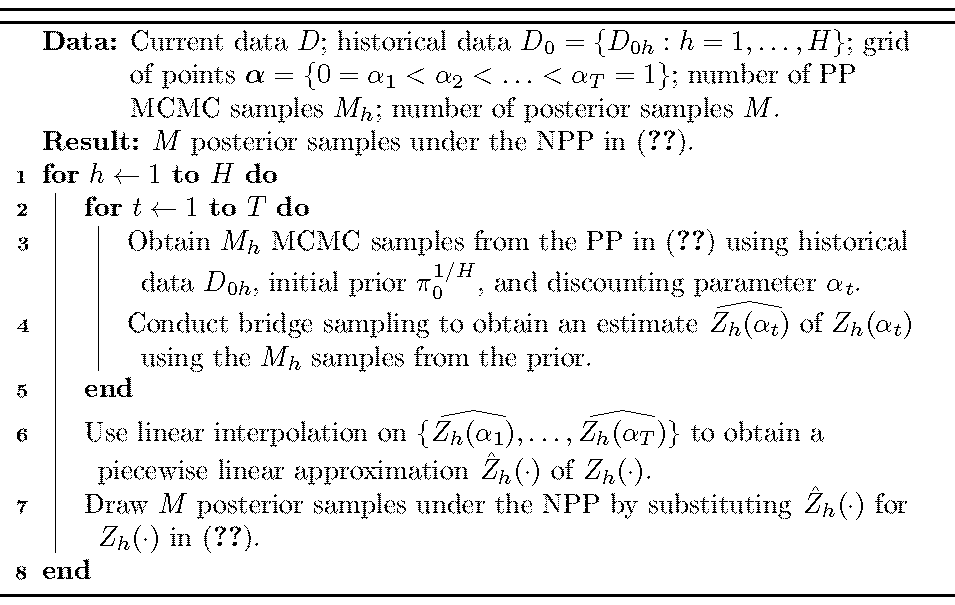
\includegraphics{alg/algnpp.png}

  \SetAlgoLined
  \KwData{Current data $D$; historical data $D_0 = \{ D_{0h}: h = 1, \ldots, H \}$; grid of points $\bm{\alpha} = \{ 0 = \alpha_1 < \alpha_2 < \ldots < \alpha_T = 1 \}$; number of PP MCMC samples $M_h$; number of posterior samples $M$.
  }
  \KwResult{$M$ posterior samples under the NPP in \eqref{eq:npp}.}

  \For{$h \leftarrow 1$ \KwTo $H$}{
    \For{$t \leftarrow 1$ \KwTo $T$}{
        Obtain $M_h$ MCMC samples from the PP in \eqref{eq:pp_fixeda0} using historical data $D_{0h}$, initial prior $\pi_0^{1/H}$, and discounting parameter $\alpha_t$.
    \\
        Conduct bridge sampling to obtain an estimate $\widehat{Z_h(\alpha_t)}$ of $Z_h(\alpha_t)$ using the $M_h$ samples from the prior.
    }
    Use linear interpolation on $\{ \widehat{Z_h(\alpha_1)}, \ldots, \widehat{Z_h(\alpha_T)} \}$ to obtain a piecewise linear approximation $\hat{Z}_h(\cdot)$ of $Z_h(\cdot)$.
    %
    \\
    Draw $M$ posterior samples under the NPP by substituting $\hat{Z}_h(\cdot)$ for $Z_h(\cdot)$ in \eqref{eq:npp}.
}
  \caption{Posterior Sampling under the Normalized Power Prior}
  \label{alg:npp}
\end{figure}

The function \code{glm.npp.lognc()} in the \CRANpkg{hdbayes} package estimates the logarithm of the normalizing constant for a single value $\alpha_{t}$ of the discounting parameter, with syntax similar to \code{stats::glm()} function. Specifically, sampling from (\ref{eq:pp_fixeda0}) is conducted via \CRANpkg{cmdstanr} and then the logarithm of the normalizing constant, $\log Z_h(\alpha_{t})$ is estimated using the \CRANpkg{bridgesampling} package.
We note that one may utilize parallel computing in order to obtain the estimated normalizing constants faster by using the \CRANpkg{parallel} package, which is included with base R. After estimating the normalizing constants $Z_h(\alpha_{t})$ over a grid of discounting parameter values, posterior samples under the NPP (\ref{eq:npp}) can be obtained using the \code{glm.npp()} function.
The syntax for this function is nearly identical to that of \code{glm.pp()} described in Section \hyperref[sec:pp]{2.2}, except that users must supply values for the arguments \code{a0.lognc} (the grid points) and \code{lognc} (the estimated logarithm of the normalizing constants) obtained as described above.

The package \CRANpkg{NPP} offers an implementation of the NPP for GLMs. \CRANpkg{NPP} uses independence or random-walk Metropolis-Hastings proposals for posterior sampling of the discounting parameters, which are fast but can be difficult to tune, often resulting in highly correlated samples \citep{robertsOptimalScalingVarious2001}. Moreover, the \CRANpkg{NPP} package uses a Laplace approximation \citep{tierney1986accurate} to estimate the normalizing constant, which is faster than the bridge sampling approach in \CRANpkg{hdbayes} but can be inaccurate in small-sample or high-dimensional settings \citep{shunLaplaceApproximationHigh1995}. Finally, each distribution in the exponential family corresponds to a separate function in \CRANpkg{NPP}, making the syntax less streamlined and somewhat cumbersome to use. 

The aforementioned \CRANpkg{BayesPPD} package also offers an implementation of the NPP. The approach is a two-step approach similar to the algorithm above. The main difference between \CRANpkg{BayesPPD} and \CRANpkg{hdbayes} besides those mentioned in Section \hyperref[sec:pp]{2.2} is that \CRANpkg{BayesPPD} conducts slice sampling to sample from the prior density (\ref{eq:pp_fixeda0}), while \CRANpkg{hdbayes} relies on HMC. 

It is worth noting that under a conjugate (multivariate normal–inverse-gamma) initial prior, the normalizing constant of the PP for the normal linear model is known and does not need to be estimated.
When users call \code{glm.npp()} with \code{family = gaussian('identity')}, the function requires them to input a grid of estimated normalizing constants. Alternatively, \CRANpkg{hdbayes} provides the \code{lm.npp()} function to sample from the posterior of a normal linear model under the NPP, which is a one-step approach that does \emph{not} require estimation of the normalizing constant before posterior sampling.

\subsection{Normalized asymptotic power prior}
\label{sec:napp}
\citet{ibrahim2000power} showed that, under large samples of the historical data set, the PP in \eqref{eq:pp_fixeda0_singledataset} converges to a multivariate normal density, i.e.,
\begin{align}
  \pi_{\text{PP}}(\bm{\beta}, \phi | D_{0h}, a_{0h}, \pi_0) \overset{n_{0h} \to \infty}{\to} \varphi\left( \bm{\beta}, \phi \left| (\hat{\bm{\beta}}_{0h}', \hat{\phi}_{0h})', ~a_{0h}^{-1} \left[ I(\hat{\bm{\beta}}_{0h}, \hat{\phi}_{0h} | D_{0h} ) \right]^{-1} \right) \right.,
  %
  \label{eq:app}
\end{align}
where $\varphi(\cdot | \bm{\mu}, \bm{\Sigma})$ is the multivariate normal density function with mean $\bm{\mu}$ and covariance matrix $\bm{\Sigma}$. Here, $\hat{\bm{\beta}}_{0h}$ and $\hat{\phi}_{0h}$ are the maximum likelihood estimates (MLEs) of $(\bm{\beta}, \phi)$ under the historical data $D_{0h}$, and $I(\cdot | D_{0h})$ is the Fisher information matrix (i.e., the expectation of the negative Hessian matrix of the log-likelihood) based on the GLM likelihood for historical data $D_{0h}$.
The right-hand side of (\ref{eq:app}) has been referred to as the ``asymptotic power prior'' \citep{ibrahim2015power}

Because the right-hand side of (\ref{eq:app}) is properly normalized, there is no need to estimate a normalizing constant if we treat $a_{0h}$ as random.
However, since the dispersion parameter $\phi$ is restricted to be positive, the normal approximation may require a large historical sample size to perform well due to potential skewness. To improve the approximation, we take the transformation $\tau = \log \phi$.
By the invariance property of MLEs, $\hat{\tau}_{0h} = \log \hat{\phi}_{0h}$, and the Jacobian matrix of this transformation is given by
$$
  J(\bm{\beta}, \tau) = \begin{pmatrix}
     \pdv{\bm{\beta}}{\bm{\beta}'} & \pdv{\bm{\beta}}{\tau} \\
     \pdv{\phi}{\bm{\beta}'}       & \pdv{\phi}{\tau}
  \end{pmatrix}
  %
  = \begin{pmatrix}
     \bm{I}  & \bm{0}_p \\
     \bm{0}_p' & \exp{\tau}
  \end{pmatrix},
$$
so that the Fisher information for historical data $D_{0h}$ is $I(\bm{\beta}, \tau) = J(\bm{\beta}, \tau)' I(\bm{\beta}, \exp\{\tau\} | D_{0h}) J(\bm{\beta}, \tau)$.

The \CRANpkg{hdbayes} package offers an implementation of what we call the normalized asymptotic power prior (NAPP) using this transformation $\tau = \log \phi$. Let $\bm{\theta} = (\bm{\beta}', \tau)'$ and $\hat{\bm{\theta}}_{0h} = (\hat{\bm{\beta}}_{0h}', \hat{\tau}_{0h})'$. The NAPP is given by
$$
\pi_{\text{NAPP}}(\bm{\theta}, \bm{a}_0 | D_0) = \prod_{h=1}^H \varphi\left( \bm{\theta} \left| \hat{\bm{\theta}}_{0h}, ~a_{0h}^{-1} [I(\hat{\bm{\theta}}_{0h} | D_{0h})]^{-1}\right) \right. \pi(a_{0h}),
$$
where we take an independent Beta prior for each $a_{0h}, h = 1, \ldots, H$.
The primary advantage of the NAPP over the NPP is that there is no need to estimate a normalizing constant, so that the implementation is a one-step approach. However, when a normal distribution is a poor approximation to the likelihood function, the NAPP might be overly informative. Posterior samples under the NAPP can be obtained using the \code{glm.napp()} function, which only requires a \code{formula}, \code{family}, and a list of \code{data.frame}s giving the current and historical data sets. To our knowledge, there are no other R packages that implement the NAPP.

\subsection{Bayesian hierarchical model}
\label{sec:bhm}

The Bayesian hierarchical model (BHM) is arguably the most widely used Bayesian model for informative prior elicitation.
The BHM assumes that the parameters for the current and historical data sets are different but come from the same distribution whose hyperparameters themselves are treated as random.

Let $(\bm{\beta}', \phi)'$ denote the GLM parameters for the current data set, where $\bm{\beta} = (\beta_1, \ldots, \beta_p)'$. Let $(\bm{\beta}_{0h}', \phi_{0h})'$ denote the GLM parameters for the historical data set $D_{0h}$, $h = 1, \ldots, H$, where $\bm{\beta}_{0h} = (\beta_{0h1}, \ldots, \beta_{0hp})'$.
The BHM as implemented in \CRANpkg{hdbayes} may be expressed hierarchically as
\begin{align}
    %% META-ANALYTIC MEAN
    \mu_j | \mu_{0j}, \sigma_{0j} &\sim N(\mu_{0j}, \sigma_{0j}^2)
        , \ \ j = 1, \ldots, p
    %
    ,\notag \\
    %% GLOBAL STDEV
    \sigma_j | m_j, s_j &\sim N^+(m_j, s_j^2)
        , \ \ j = 1, \ldots, p
    % PRIORS FOR REGRESSION COEFFICIENTS
    ,\notag \\
    \beta_j, \beta_{0hj} | \mu_j, \sigma_j &\overset{\text{i.i.d.}}{\sim} N(\mu_j, \sigma_j^2)
        , \ \ h = 1, \ldots, H
        , \ \ j = 1, \ldots, p
    % PRIORS FOR DISPERSION PARAMETERS
    ,\notag \\
    \phi | m_0, s_0 &\sim N^{+}(m_0, s_0^2)
        , \notag \\
    \phi_{0h} | m_{0h}, s_{0h} &\sim N^{+}(m_{0h}, s_{0h}^2)
        , \ \  h = 1, \ldots, H
    % LIKELIHOOD FOR CURRENT
    ,\notag \\
    y_i    | \bm{\beta}, \phi &\sim f(y_i | \bm{\beta}, \phi)
        , \ \ i = 1, \ldots, n
    % LIKELIHOOD FOR HISTORICAL
    , \notag \\
    y_{0hi} | \bm{\beta}_{0h}, \phi_{0h} &\sim f(y_{0hi} | \bm{\beta}_{0h}, \phi_{0h}), 
        \ \ h = 1, \ldots, H, 
        \ \ i = 1, \ldots, n_{0h}, 
    \label{eq:bhm}
\end{align}
where $f(\cdot | \bm{\beta}, \phi)$ is the density (or mass) function corresponding to the GLM likelihood in \eqref{eq:glm_likelihood}. Here, $\mu_j$ is referred to as the global (or meta-analytic) mean, $\sigma_j$ is the global standard deviation (which measures the heterogeneity of parameters across data sets), and $\bm{\xi} = ( m_0, s_0, \{(m_{0h}, s_{0h}): h = 1, \ldots, H \}, \{ (\mu_{0j}, \sigma_{0j}, m_j, s_j): j = 1, \ldots, p \} )$ denotes the collection of elicited hyperparameters.
The hyperparameters $s_j$ are the most crucial ones, as they must often be chosen to be somewhat subjective and reflect most of the borrowing properties under the BHM.

Let $\bm{\theta}$ denote all parameters to be sampled in \eqref{eq:bhm}. The posterior density of \eqref{eq:bhm} can be expressed as
\begin{align}
    p_{\text{BHM}}(\bm{\theta} | D, D_0, \bm{\xi}) \propto
    L(\bm{\beta}, \phi | D)
    \left[
        \prod_{h=1}^H L(\bm{\beta}_{0h}, \phi_{0h} | D_{0h})
    \right]
    \pi_{\text{BHM}}(\bm{\theta})
    %
    ,
    \label{eq:bhm_post}
\end{align}
where
\begin{align}
    \pi_{\text{BHM}}(\bm{\theta}) &=
    \varphi^+(\phi | m_0, s_0^2)
    \left[ \prod_{h=1}^H \varphi^+(\phi_{0h} | m_{0h}, s_{0h}^2) \right] \cdot \notag \\
    &~~~~~ \left\{
    \prod_{j=1}^p 
    \left[ \varphi(\mu_j | \mu_{0j}, \sigma_{0j}^2) \varphi^+(\sigma_j | m_j, s_j^2)
    \varphi(\beta_j | \mu_j, \sigma_j^2) \prod_{h=1}^H \varphi(\beta_{0hj} | \mu_j, \sigma_j^2)
    \right]
    \right\},
    %
    \label{eq:bhm_prior}
\end{align}
and $\varphi^+(\cdot | a, b^2)$ denotes the density of a truncated normal distribution $N^{+}(a, b^2)$. 

In \CRANpkg{hdbayes}, posterior inference under the BHM can be conducted using the \code{glm.bhm()} function. The default hyperparameters values are $\mu_{0j} = 0$, $\sigma_{0j} = 10$, $m_j = 0$, $s_j = 1$, $m_0 = m_{0h} = 0$, $s_0 = s_{0h} = 10$ for $j = 1, \ldots, p$ and $h = 1, \ldots, H$. The value $s_j = 1$ is moderately informative but is designed to encourage information borrowing. In general, $s_j$ cannot be chosen to be large unless there are many ($e.g. \ge 10$) historical data sets, which is rarely the case. 

Several R packages provide related functionality for hierarchical modeling. The R package \CRANpkg{historicalborrow} implements hierarchical models for borrowing information from historical studies. However, it assumes continuous (normal) outcomes and focuses on borrowing information only on the mean outcome of the control arm, whereas \CRANpkg{hdbayes} supports a broad class of GLMs and enables leveraging information on both control and treatment arms as well as on covariate effects. A BHM similar to that implemented in \CRANpkg{hdbayes} can also be fitted using the \code{gMAP()} function in the \CRANpkg{RBesT} package. Although the documentation and vignettes of \CRANpkg{RBesT} primarily illustrate \code{gMAP()} for deriving a prior from historical data, the same function can, in principle, be used to obtain posterior inference from a BHM by including the current trial as an additional study within the hierarchical model. \CRANpkg{RBesT} supports GLMs for normal, binomial, and Poisson outcomes, but it is designed for aggregate (study-level) data and does not directly accommodate covariate adjustment. In contrast, \CRANpkg{hdbayes} accommodates individual-level data and naturally incorporates covariates as in \code{stats::glm()} function.

\subsection{2.6 Robust meta-analytic predictive prior}
\label{sec:RMAP}

The \emph{robust} meta-analytic predictive (RMAP) prior \citep{schmidli2014robust} extends the BHM framework introduced in Section~\hyperref[sec:bhm]{2.5} by incorporating a vague (non-informative) component to mitigate prior–data conflict. As shown by \citet{schmidli2014robust}, the BHM in \eqref{eq:bhm_post} induces a prior for the regression coefficients of the current study, referred to as the meta-analytic predictive (MAP) prior, which is given by
\begin{align}
    \pi_{\text{MAP}}(\bm{\beta} | D_0)
        &= \int \int \left[\prod_{j=1}^p \varphi(\beta_j | \mu_j, \sigma_j^2) \right] \pi(\bm{\mu}, \bm{\sigma} | D_0) d\bm{\mu} d\bm{\sigma},
        %
        \label{eq:map}
\end{align}
where $\bm{\mu} = (\mu_1, \ldots, \mu_p)$, $\bm{\sigma} = (\sigma_1, \ldots, \sigma_p)$, and $\pi(\bm{\mu}, \bm{\sigma} | D_0)$ is the posterior density of $(\bm{\mu}, \bm{\sigma})$ obtained by fitting a BHM to the historical data only, i.e.,
\begin{align}
    \pi(\bm{\mu}, \bm{\sigma} | D_0) &= 
    \int \int p_{\text{BHM}}(\bm{\mu}, \bm{\sigma}, \bm{\beta}_0, \bm{\phi}_0 | D_0) d\bm{\beta}_0 d\bm{\phi}_0
    ,\notag \\
    &\propto \int \int \left\{\prod_{h=1}^H L(\bm{\beta}_{0h}, \phi_{0h} | D_{0h}) \varphi^+(\phi_{0h} | m_{0h}, s_{0h}^2) \prod_{j=1}^p \varphi(\beta_{0hj} | \mu_j, \sigma_j^2)
    \right\}
    \notag\\
    &\qquad\qquad \cdot
    \left\{\prod_{j=1}^p
      \varphi(\mu_j | \mu_{0j}, \sigma_{0j}^2)\,
      \varphi^+(\sigma_j | m_j, s_j^2)
    \right\} d\bm{\beta}_0\, d\bm{\phi}_0,
    %
    \label{eq:map_mean_sd}
\end{align}
where $p_{\text{BHM}}(\cdot | D_0)$ denotes the posterior density of the BHM for the historical data given in \eqref{eq:bhm_post}, $\bm{\beta}_0 = (\bm{\beta}_{01}', \ldots, \bm{\beta}_{0H}')'$, and $\bm{\phi}_0 = (\phi_{01}, \ldots, \phi_{0H})'$.

The RMAP prior is constructed as a two-component mixture of the MAP prior and a vague prior. For an arbitrary parameter vector $\bm{\theta}$, the RMAP prior is defined as 
$$\pi_{\text{RMAP}}(\bm{\theta} | D_0, \gamma) = \gamma \pi_{\text{MAP}}(\bm{\theta} | D_0) + (1 - \gamma) \pi_{v}(\bm{\theta}),$$
where $\gamma \in [0, 1]$ is an elicited hyperparameter that controls the degree of borrowing from the historical data, and $\pi_v$ denotes the vague prior. When $\gamma = 0$, the RMAP prior reduces to the vague prior, whereas when $\gamma = 1$, it is identical to the MAP prior, yielding the same posterior distribution as the BHM when combined with the current data likelihood.

Although \cite{schmidli2014robust} recommends approximating the MAP prior using a finite mixture of conjugate priors, it can be difficult and time-consuming to identify an appropriate approximation. The \CRANpkg{RBesT} package implements this approach using the expectation–maximization (EM) algorithm, which enables fast analytic posterior computation and facilitates the evaluation of operating characteristics in trial designs based on the RMAP prior. In contrast, \CRANpkg{hdbayes} does not rely on finite-mixture approximations. Instead, it computes the posterior under the RMAP prior by directly evaluating the marginal likelihoods of the vague and MAP priors. Specifically, the posterior under the RMAP prior is given by
\begin{align}
    p_{\text{RMAP}}(\bm{\beta}, \phi | D, D_0, \gamma) &= 
    \frac{
    L(\bm{\beta}, \phi | D) \left[ \gamma \pi_I(\bm{\beta}, \phi | D_0) + (1 - \gamma) \pi_V(\bm{\beta}, \phi) \right]
    }{
        \int \int
        L(\bm{\beta}^*, \phi^* | D) \left[ \gamma \pi_I( \bm{\beta}^* \phi^* | D_0) + (1 - \gamma) \pi_V( \bm{\beta}^*, \phi^* ) \right] 
        d\bm{\beta}^*, d\phi^*
    }
    ,
    \notag \\
    &= \tilde{\gamma} p_I(\bm{\beta}, \phi | D, D_0) + (1 - \tilde{\gamma}) p_V(\bm{\beta}, \phi | D),
\end{align}
where $p_I(\bm{\beta}, \phi | D, D_0) = L(\bm{\beta}, \phi | D) \pi_I(\bm{\beta}, \phi | D_0) / Z_I(D, D_0)$ is the posterior density under the informative (MAP) prior, $p_V(\bm{\beta}, \phi | D) = L(\bm{\beta}, \phi | D) \pi_V(\bm{\beta}, \phi) / Z_V(D)$ is the posterior density under the vague prior, and
\begin{align}
    \tilde{\gamma} = \frac{ \gamma Z_I(D, D_0) }{ \gamma Z_I(D, D_0) + (1 - \gamma) Z_V(D) }
    %
    \label{eq:rmap_weight}
\end{align}
is the updated mixture weight. The normalizing constants $Z_I(D, D_0)$ and $Z_V(D)$ are estimated via the \CRANpkg{bridgesampling} package within \CRANpkg{hdbayes}. This approach obviates the need for finite-mixture approximations of the MAP prior and is often more computationally convenient. Details for computing the normalizing constants are provided in Section \hyperref[sec:normconst]{3}. The procedure for obtaining posterior samples under the RMAP prior is summarized in Algorithm \ref{alg:rmap}.

\begin{figure}
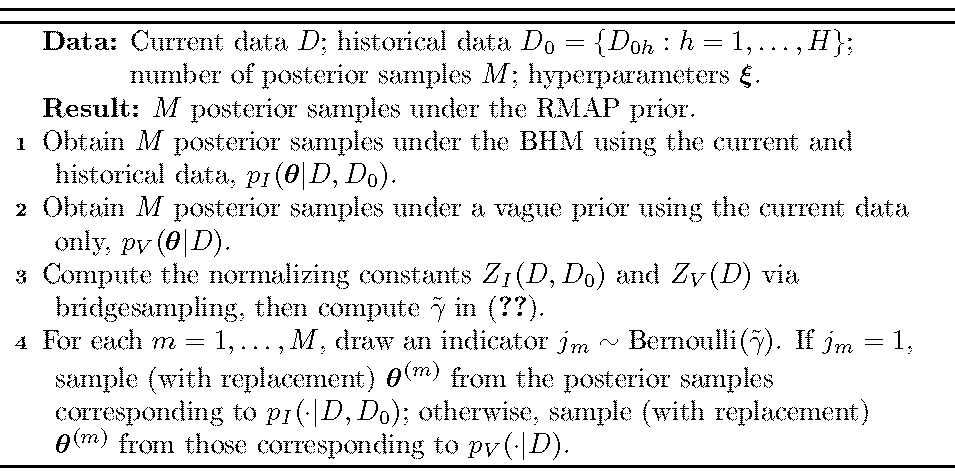
\includegraphics{alg/algrmap.png}

  \SetAlgoLined
  \KwData{Current data $D$; historical data $D_0 = \{ D_{0h}: h = 1, \ldots, H \}$; number of posterior samples $M$; hyperparameters $\bm{\xi}$.
  }
  \KwResult{$M$ posterior samples under the RMAP prior.}
  Obtain $M$ posterior samples under the BHM using the current and historical data, $p_{I}(\bm{\theta} | D, D_0)$.
  \\ Obtain $M$ posterior samples under a vague prior using the current data only, $p_V(\bm{\theta} | D)$.
  %
  \\ Compute the normalizing constants $Z_I(D, D_0)$ and $Z_V(D)$ via \CRANpkg{bridgesampling}, then compute $\tilde{\gamma}$ in \eqref{eq:rmap_weight}.
  %
  \\ For each $m = 1, \ldots, M$, draw an indicator $j_m \sim \text{Bernoulli}(\tilde{\gamma})$. If $j_m = 1$, sample (with replacement) $\bm{\theta}^{(m)}$ from the posterior samples corresponding to $p_I(\cdot | D, D_0)$; otherwise, sample (with replacement) $\bm{\theta}^{(m)}$ from those corresponding to $p_V(\cdot | D)$.
  \caption{Posterior Sampling under the Robust Meta-Analytic Predictive Prior}
  \label{alg:rmap}
\end{figure}

\subsection{Commensurate prior}
\label{sec:cp}

The commensurate prior (CP) of \cite{hobbs2012commensurate} is a hierarchical prior. In the traditional CP, the current data regression coefficients, $\bm{\beta} = (\beta_1, \ldots, \beta_p)'$, are assumed to follow normal distributions centered at the historical data regression coefficients, $\bm{\beta}_0 = (\beta_{01}, \ldots, \beta_{0p})'$, with hierarchical precision parameters. Specifically, the CP assumes $\beta_j \sim N(\beta_{0j}, \tau_j^{-1})$, where $\tau_j$ is referred to as the ``commensurability parameter'' for the $j^{th}$ regression coefficient. The parameter $\tau_j$ measures how compatible the current and historical data are based on the $j^{th}$ covariate, with larger values indicating a higher degree of commensurability.

To our knowledge, a CP for multiple historical data sets has not yet been formally developed. In \CRANpkg{hdbayes}, we implement the CP by assuming that all historical data sets share the same regression coefficients (but may have different dispersion parameters, if applicable).
Expressed hierarchically, the CP as implemented in \CRANpkg{hdbayes} is given by
\begin{align}
    %
   &\beta_{0j} | \mu_{0j}, \sigma_{0j} \sim N(\mu_{0j}, \sigma_{0j}^2), \ \ j = 1, \ldots, p
   %
   , \notag \\
   &\phi | m_0, s_0 \sim N^+(m_0, s_0^2)
   %
   ,\notag \\
   &\phi_{0h} | m_{0h}, s_{0h} \sim N^+(m_{0h}, s_{0h}^2), \ \ h = 1, \ldots, H 
   %
   ,\notag \\
   %\tau_j | \eta_{0j}, \omega_{0j} &\sim N^+(\eta_{0j}, \omega_{0j}^2), \ \ j = 1, \ldots, p
   %, \notag \\
   &\beta_j | \beta_{0j}, \tau_j \sim N\left( \beta_{0j}, \tau_j^{-1} \right),
        \ \ j = 1, \ldots, p
    %
    ,\notag \\
    &\tau_j | p_{\text{spike}}, \mu_{\text{spike}}, \sigma_{\text{spike}}, \mu_{\text{slab}}, \sigma_{\text{slab}} \sim 
    p_{\text{spike}} N^+(\mu_\text{spike}, \sigma_{\text{spike}}^2)
    + (1 - p_{\text{spike}}) N^+(\mu_{\text{slab}}, \sigma_{\text{slab}}^2)
    %
    , \notag \\
    &y_i    | \bm{\beta}, \phi \sim f(y_i | \bm{\beta}, \phi), \ \  i = 1, \ldots, n
    %
    , \notag \\
    &y_{0hi} | \bm{\beta}_0, \phi_{0h} \sim f(y_{0hi} | \bm{\beta}_0, \phi_{0h}), \ \ h = 1, \ldots, H, \ \  i = 1, \ldots, n_{0h}.
    %
    \label{eq:comm_hm}
\end{align}
Following \citet{hobbs2012commensurate}, we elicit a spike-and-slab prior on the commensurability parameters $\tau_j$.
When there is only one historical data set ($H = 1$), the CP implemented in \CRANpkg{hdbayes} corresponds to the traditional CP of \citet{hobbs2012commensurate}. 

The CP is implemented in \CRANpkg{hdbayes} via the function \code{glm.commensurate()}.
The default hyperparameters are
\begin{align*}
    \mu_{0j} &= 0, \ \ j = 1, \ldots, p
    ,\\
    \sigma_{0j} &= 10, \ \ j = 1, \ldots, p
    ,\\
    m_0 &= m_{0h} = 0, \ \ h = 1, \ldots, H
    , \\
    s_0 &= s_{0h} = 10, \ \ h = 1, \ldots, H
    , \\
    p_{\text{spike}} &= 0.1
    ,\\
     \mu_{\text{spike}} &= 200
    ,\\
    \sigma_{\text{spike}} &= 0.1
    , \\
    \mu_{\text{slab}} &= 0
    , \\
    \sigma_{\text{slab}} &= 5.
\end{align*}
The default ``spike'' component approximates a point mass at $\tau_j = 200$, encouraging a high degree of borrowing, whereas the default ``slab'' component is a half-normal distribution with scale 5, which places most of its mass on smaller values of $\tau_j$, allowing a smaller amount of borrowing. In general, eliciting hyperparameters for the spike-and-slab prior on the $\tau_j$'s is problem specific.

The R packages \CRANpkg{psborrow} \citep{psborrow_pkg} and \CRANpkg{psborrow2} \citep{psborrow2_pkg} provide propensity score-based implementations of the CP, with the former relying on \CRANpkg{rjags} to conduct MCMC sampling and the latter relying on \CRANpkg{cmdstanr} (as does \CRANpkg{hdbayes}). 
The \CRANpkg{psborrow2} package offers more flexibility in specifying initial priors than \CRANpkg{hdbayes}. However, since initial priors are usually taken to be non-informative, the class of prior distributions has little impact on the analysis results in the vast majority of applications.
Moreover, this increased flexibility comes at the cost of a more complicated syntax, while the syntax in \CRANpkg{hdbayes} is similar to the \texttt{glm} function in the \CRANpkg{stats} package.

\subsection{Latent exchangeability prior}\label{sec:LEAP}
The latent exchangeability prior (LEAP), developed by \citet{alt2023leap}, assumes that the historical data are generated from a finite mixture model consisting of $K \ge 2$ components, with the current data generated from one component of this mixture (taken to be the first component, without loss of generality). For a single historical data set, the posterior under the LEAP can be expressed hierarchically as
\begin{align}
    \bm{\gamma} &\sim \text{Dirichlet}(\bm{\alpha}_0)
    ,\notag \\
    %
    \bm{\beta}, \bm{\beta}_{0k} 
        &\overset{\text{i.i.d.}}{\sim}
        N(\bm{\mu}_0, \bm{\Sigma}_0)
    , \ \ k = 2, \ldots, K
    ,\notag \\
    %
    \phi, \phi_{0k}
        &\overset{\text{i.i.d.}}{\sim}
        N^+(m_0, s_0^2)
    , \ \ k = 2, \ldots, K
    ,\notag \\
    %
    y_i | \bm{\beta}, \phi &\sim f(\cdot | \bm{\beta}, \phi)
    , \ \  i = 1, \ldots, n
    , \notag \\
    %
    y_{0i} | \bm{\beta}, \bm{\beta}_0, \phi, \bm{\phi}_0, \bm{\gamma} &\sim \gamma_1 f(\cdot | \bm{\beta}, \phi) + \sum_{k=2}^K \gamma_k f(\cdot | \bm{\beta}_{0k}, \phi_{0k}), 
    , \ \ i = 1, \ldots, n_0,
    %
    \label{eq:leap}
\end{align}
where $\bm{\gamma} = (\gamma_1, \ldots, \gamma_K)$ are the mixing probabilities, and $\bm{\alpha}_0 = (\alpha_{01}, \ldots, \alpha_{0K})'$ is the concentration hyperparameter of the Dirichlet prior. The prior mean and covariance for the $K$ regression coefficients are denoted by $\bm{\mu}_0$ and $\bm{\Sigma}_0$, respectively, while $m_0$ and $s_0$ are the location and scale parameters of the truncated normal prior on the $K$ dispersion parameters. The default hyperparameters in \CRANpkg{hdbayes} are $K = 2$, $\bm{\alpha}_0 = \bm{1}_K$, $\bm{\mu}_0 = \bm{0}_p$, $\bm{\Sigma}_0 = \text{diag}\{ \sigma_{0j}^2, j = 1, \ldots p \}$ with $\sigma_{0j} = 10$, corresponding to non-informative initial priors.

Unlike the priors described above, which conduct blanket discounting of the historical data, the LEAP conducts discounting at the individual level of the historical data. Since the LEAP has not been developed for multiple historical data sets, the approach taken by \CRANpkg{hdbayes} is to stack all $H$ historical data sets into a single combined data set $D_0$ with $n_0 = \sum_{h=1}^H n_{0h}$ observations. The LEAP is implemented via the \code{glm.leap()} function in \CRANpkg{hdbayes}, which provides the first implementation of the LEAP in a publicly available R package.

\section{Model selection via marginal likelihoods}\label{sec:normconst}
Canonical Bayesian model selection proceeds by calculating the marginal likelihood (also referred to as the ``evidence''). For example, suppose the model space $\mathcal{M} = \{M_1, M_2\}$ consists of two candidate models. \cite{kass1995bayes} shows that the preference of $M_2$ over $M_1$ can be expressed in terms of the Bayes factor, given by
\begin{align}
    \text{BF}(D) = \frac{Z_2(D)}{Z_1(D)} = \frac{ \int L_2(\bm{\theta}_2 | D) \pi_2(\bm{\theta}_2) d\bm{\theta}_2 }{ \int L_1(\bm{\theta}_1 | D) \pi_1(\bm{\theta}_1) d\bm{\theta}_1 },
\end{align}
where $L_j(\cdot | D)$ is the likelihood corresponding to model $M_j$ with parameters $\bm{\theta}_j$ and prior $\pi_j$, and $Z_j(D)$ is the normalizing constant of the posterior for model $M_j$ and prior $\pi_j$ (i.e., the marginal likelihood for model $M_j$). 

In \CRANpkg{hdbayes}, many of the implemented priors are not normalized. While this does not present an issue for accurate MCMC sampling, it generally leads to marginal likelihoods that are only accurate up to a constant of proportionality. When comparing models with different priors, regression coefficients, etc., this can result in incorrect Bayes factors. Let $\pi(\bm{\theta}) = \tilde{\pi}(\bm{\theta}) / C$ denote a prior for $\bm{\theta}$, where $\tilde{\pi}$ is the unnormalized prior, and $C = \int \tilde{\pi}(\bm{\theta}) d\bm{\theta}$ is its normalizing constant. The marginal likelihood may be computed as
\begin{align}
    Z(D) &= \int L(\bm{\theta} | D) \pi(\bm{\theta}) d\bm{\theta}
    %
    = \frac{ \int L(\bm{\theta} | D) \tilde{\pi}(\bm{\theta}) d\bm{\theta} }{ \int \tilde{\pi}(\bm{\theta}^*) d\bm{\theta}^* }
    %
    = \frac{\tilde{Z}(D)}{C},
    %
    \label{eq:normconst}
\end{align}
where $\tilde{Z}(D) = \int L(\bm{\theta} | D) \tilde{\pi}(\bm{\theta}) d\bm{\theta}$. 

It follows that the marginal likelihood can be computed in a two-step process. First, the normalizing constant of the unnormalized prior is estimated, for example, via bridge sampling using MCMC samples from the prior. Second, MCMC samples are drawn from the posterior under $\tilde{\pi}$, and the normalizing constant of the posterior is then estimated, again via bridge sampling. The ratio of these two estimates gives the marginal likelihood $Z(D)$.

We give an example of these techniques in Appendix \hyperref[sec:app_link_selection]{A}, where we illustrate how to select between the logit and probit link functions for the HIV data set (see Section~\hyperref[sec:dataanalysis_logistic]{4.1}) under the PP using the marginal likelihood functionality in \CRANpkg{hdbayes}. 

\subsection{Example: LEAP}
To illustrate our approach, consider the LEAP. Let $L(\bm{\theta}_1 | D)$ denote the likelihood for the current data, and let $L_0(\bm{\theta}, \bm{\gamma} | D_0)$ denote the likelihood pertaining to the mixture model for the historical data, where $\bm{\theta} = (\bm{\theta}_1', \ldots, \bm{\theta}_K')'$ and $\bm{\gamma} = (\gamma_1, \ldots, \gamma_K)'$. Also, let $\pi_0(\bm{\theta}, \bm{\gamma})$ denote the initial prior. The marginal likelihood under the LEAP can be expressed as
\begin{align}
    Z(D) &= \int L(\bm{\theta}_1 | D) \pi_\text{LEAP}(\bm{\theta}_1 | D_0) d\bm{\theta}_1, \notag \\
    % %
    % = \int \int L(\bm{\theta}_1 | D) \pi_\text{LEAP}( \bm{\theta}, \bm{\gamma} | D_0) d\bm{\theta} d\bm{\gamma}
    %
    % ,\notag \\ &
    &= \int \int L(\bm{\theta}_1 | D) \frac{ L_0(\bm{\theta}, \bm{\gamma} | D_0)) \pi_0(\bm{\theta}, \bm{\gamma})  }{ \int \int L_0(\bm{\theta}^*, \bm{\gamma}^* | D_0) d\bm{\theta}^* d\bm{\gamma}^* } d\bm{\theta} d\bm{\gamma}
    %
    ,\notag \\ 
    &= \frac{ \int \int L(\bm{\theta}_1 | D) L_0(\bm{\theta}, \bm{\gamma} | D_0) \pi_0(\bm{\theta}, \bm{\gamma}) d\bm{\theta} d\bm{\gamma} }
    {\int \int L_0(\bm{\theta}^*, \bm{\gamma}^* | D_0) d\bm{\theta}^* d\bm{\gamma}^*},
    %
    \label{eq:normconst_leap}
\end{align}
which takes the same form as \eqref{eq:normconst}. To estimate the marginal likelihood under the LEAP in \CRANpkg{hdbayes}, users first fit the LEAP using the \code{glm.leap()} function. The resulting fitted object is then passed to \code{glm.logml.leap()}, which internally performs two bridge-sampling steps. First, it draws MCMC samples from the prior and computes the normalizing constant of the prior (the denominator in \eqref{eq:normconst_leap}). Then, it estimates the normalizing constant of the posterior (the numerator in \eqref{eq:normconst_leap}). The ratio of these two quantities provides the marginal likelihood $Z(D)$ under the LEAP.

The function can be called as
\begin{verbatim}
    glm.logml.leap(post.samples, bridge.args, ...)
\end{verbatim}
where \code{post.samples} is the fitted object returned by \code{glm.leap()}, \code{bridge.args} is a list of arguments passed to \code{bridgesampling::bridge\_sampler()}, and \code{...} includes additional arguments for the \CRANpkg{cmdstanr} sampler used to draw prior samples for estimating the denominator in \eqref{eq:normconst_leap}. 

Analogous functions for other priors are available in \CRANpkg{hdbayes}, including \code{glm.logml.pp()} (PP), \code{glm.logml.npp()} (NPP), \code{glm.logml.napp()} (NAPP), and \code{glm.logml.map()} (BHM). For the NPP and NAPP, the priors are already normalized, so no estimation of the prior normalizing constant is required. A separate function for the RMAP prior is not provided, but its marginal likelihood can be easily computed using the updated mixture weight in \eqref{eq:rmap_weight} (included in the output of \code{glm.rmap()}) and the marginal likelihoods under the MAP and vague priors. 

\section{Data analyses}
\label{sec:dataanalysis}
\subsection{4.1 Logistic regression example}
\label{sec:dataanalysis_logistic}

We now illustrate the functionality in \CRANpkg{hdbayes} by analyzing the data on two clinical trials presented in Section 4.2 of \citet{chen1999prior} using logistic regression to model progression to HIV in a cohort of patients treated with zidovudine (AZT). 
More details and full output can be found in the vignette ``AIDS-Progression`` that accompanies \CRANpkg{hdbayes}. The historical data come from the ACTG019 study \citep{Volberding1990}, which
was a double-blind placebo-controlled clinical trial comparing AZT with a placebo in people with CD4 cell counts below 500.
The sample size of complete observations for this study was $n_0 = 822$.
The response variable (\code{outcome}) is binary, taking the value 1 for death,
development of AIDS or AIDS-related complex (ARC) and 0 otherwise.
The covariates considered are CD4 cell count (\code{cd4}), \code{age}, \code{treatment} and
\code{race}.

Our goal is to analyze data from a more recent study, ACTG036 \citep{Merigan1991}, which includes $n=183$ observations. We use the methods implemented in \CRANpkg{hdbayes} to construct informative priors based on the ACTG019 study (historical data) and apply them to the analysis of ACTG036, using the same set of covariates. To facilitate computation, we center and scale the continuous covariates (\code{age} and \code{cd4}).
In general, we recommend this preprocessing step in order to keep regression coefficients on roughly the same scale and thus avoid difficult posterior geometries for the Stan dynamic Hamiltonian Monte Carlo (dHMC) procedure to explore.
The data preparation can be accomplished by calling
\begin{verbatim}
library(hdbayes)
library(posterior)
library(dplyr)
library(parallel)

data(actg019)
data(actg036)
age_stats <- with(actg036,
                  c('mean' = mean(age), 'sd' = sd(age)))
cd4_stats <- with(actg036,
                  c('mean' = mean(cd4), 'sd' = sd(cd4)))
actg036$age <- ( actg036$age - age_stats['mean'] ) / age_stats['sd']
actg019$age <- ( actg019$age - age_stats['mean'] ) / age_stats['sd']
actg036$cd4 <- ( actg036$cd4 - cd4_stats['mean'] ) / cd4_stats['sd']
actg019$cd4 <- ( actg019$cd4 - cd4_stats['mean'] ) / cd4_stats['sd']

\end{verbatim}
Now, we set up the analysis by creating a formula and (GLM) family, as well as obtaining the maximum likelihood estimates (MLEs) of the regression coefficients in both current and historical data models using \code{stats::glm()}. We also specify a list of data sets, with the first element being the current data and the second element being the historical data. In \CRANpkg{hdbayes}, we assume that the first specified data set in the list is the current data set, and any other data sets are historical.
\begin{verbatim}
formula <- outcome ~  age + race + treatment + cd4
p       <- length(attr(terms(formula), "term.labels")) ## number of predictors
family  <- binomial('logit')

fit.mle.cur  <- glm(formula, family, actg036)
fit.mle.hist <- glm(formula, family, actg019)

the.data <- list(actg036, actg019)
\end{verbatim}
We can now briefly inspect the confidence intervals for the coefficients in the historical data (ACTG019) model:
\begin{verbatim}
round(confint(fit.mle.hist), 3)

             2.5 % 97.5 %
(Intercept) -6.901 -2.440
age          0.114  0.870
race        -0.026  4.424
treatment   -1.357 -0.158
cd4         -1.031 -0.396
\end{verbatim}
and for the coefficients in the current data (ACTG036) model:
\begin{verbatim}
round(confint(fit.mle.cur), 3)

             2.5 % 97.5 %
(Intercept) -7.237 -1.840
age         -0.513  0.813
race        -1.932  3.141
treatment   -1.575  1.317
cd4         -2.913 -0.926
\end{verbatim}
From these confidence intervals, we observe (i) substantial uncertainty in the coefficient estimates from the current data model and (ii) notable discrepancies between the estimates from the current and historical data models, particularly for \code{treatment}, which is of primary interest. This motivates the use of informative priors that leverage historical data while accommodating potential prior-data conflict by allowing for discounting.

Next, we set up the computational specifications for our analysis, in which we will run four parallel Markov chains, each with {2,500} posterior samples following a burn-in period of {1,000} iterations (yielding a total of {10,000} post-burn-in samples):

\begin{verbatim}
ncores        <- 4
nchains       <- 4 ## number of Markov chains
iter_warmup   <- 1000 ## warmup per chain for MCMC sampling
iter_sampling <- 2500 ## number of samples post warmup per chain
\end{verbatim}
We are now prepared to fit the BHM (Section~\hyperref[sec:bhm]{2.5}), which can be achieved by simply calling its dedicated function, \code{glm.bhm()}:

\begin{verbatim}
fit.bhm <- glm.bhm(
  formula, family, the.data,
  meta.mean.mean = 0, meta.mean.sd = 10,
  meta.sd.mean = 0, meta.sd.sd = 0.5,
  iter_warmup = iter_warmup, iter_sampling = iter_sampling,
  chains = nchains, parallel_chains = ncores,
  refresh = 0
)
\end{verbatim}
The output from \code{glm.bhm()} is a \code{draws\_df} object derived from the \CRANpkg{posterior} package \citep{posterior_pkg}. One may utilize functions in the \CRANpkg{posterior} package, like \code{summarise\_draws()}, to acquire posterior inference and MCMC diagnostics. For instance, one can obtain posterior mean, standard deviation, and quantiles for both current and historical data regression coefficients as follows:

\begin{verbatim}
## function to pull out the summaries in a convenient form
## function to pull out the posterior summaries in a convenient form
get_summaries <- function(fit, pars.interest, digits = 3) {
    fit %>%
      select(all_of(pars.interest)) %>%
      summarise_draws(mean, sd, ~quantile(.x, probs = c(0.025, 0.5, 0.975)),
                      .num_args = list(digits = digits))
}
## names of current and historical regression: coefficients
base.pars      <- c("(Intercept)", "age", "race", "treatment", "cd4")
base.pars.hist <- paste(base.pars, "hist", "1", sep="_")
get_summaries(fit = fit.bhm, pars.interest = c(base.pars, base.pars.hist))

# A tibble: 10 × 6
   variable             mean    sd `2.5%`  `50%` `97.5%`
   <chr>               <dbl> <dbl>  <dbl>  <dbl>   <dbl>
 1 (Intercept)        -4.130 0.906 -6.151 -4.049  -2.601
 2 age                 0.262 0.261 -0.307  0.283   0.729
 3 race                1.012 0.903 -0.593  0.958   2.956
 4 treatment          -0.644 0.430 -1.496 -0.648   0.231
 5 cd4                -1.247 0.369 -2.066 -1.214  -0.645
 6 (Intercept)_hist_1 -3.917 0.828 -5.791 -3.841  -2.527
 7 age_hist_1          0.456 0.185  0.097  0.455   0.822
 8 race_hist_1         1.383 0.826  0.006  1.309   3.267
 9 treatment_hist_1   -0.706 0.291 -1.287 -0.700  -0.139
10 cd4_hist_1         -0.776 0.164 -1.098 -0.777  -0.450
\end{verbatim}

Although not shown above, the \code{posterior::summarise\_draws()} function can also be used to compute common MCMC convergence and efficiency diagnostics, such as the R-hat statistic, bulk effective sample size (bulk-ESS), and tail effective sample size (tail-ESS). For example, 
\begin{verbatim}
posterior::summarise_draws(fit.bhm, rhat, ess_bulk, ess_tail)
\end{verbatim}
All model-fitting functions in \CRANpkg{hdbayes} (e.g., \code{glm.bhm()}, \code{glm.pp()}, \code{glm.leap()}) return objects of class \code{draws\_df}, which can be directly passed to functions in the \CRANpkg{bayesplot} package \citep{bayesplot_pkg} to visualize MCMC diagnostics, such as trace plots and autocorrelation (ACF) plots. This feature allows users to leverage existing tools to assess MCMC convergence and mixing without the need for additional diagnostic functions within \CRANpkg{hdbayes}. For example, one can generate trace plots for selected coefficients using 
\begin{verbatim}
    bayesplot::mcmc_trace(fit.bhm, pars = c("age", "race", "treatment", "cd4"))
\end{verbatim}
and ACF plots using
\begin{verbatim}
    bayesplot::mcmc_acf(fit.bhm, pars = c("age", "race", "treatment", "cd4"))
\end{verbatim}
Together, the functions in \CRANpkg{posterior} and \CRANpkg{bayesplot} provide a straightforward and comprehensive approach for conducting MCMC diagnostics for all models implemented in \CRANpkg{hdbayes}.

Having used the BHM as an example of the type of output that can be obtained from functions available in \CRANpkg{hdbayes}, we now illustrate how to fit the other models introduced in Section~\hyperref[sec:priorelicit]{2} to enable later comparison of their results. To fit the CP (Section~\hyperref[sec:cp]{2.7}), one can simply call \code{glm.commensurate()}. Posterior inference for the current and historical data regression coefficients can then be obtained in the same manner as in the BHM example.

\begin{verbatim}
fit.commensurate <- glm.commensurate(
  formula = formula, family = family, data.list = the.data,
  p.spike = 0.1, spike.mean = 200, spike.sd = 0.1,
  slab.mean = 0, slab.sd = 5,
  iter_warmup = iter_warmup, iter_sampling = iter_sampling,
  chains = nchains, parallel_chains = ncores,
  refresh = 0
)
base.pars.hist <- paste(base.pars, "hist", sep="_")
get_summaries(fit = fit.commensurate, pars.interest = c(base.pars, base.pars.hist))

# A tibble: 10 × 6
   variable           mean    sd `2.5%`  `50%` `97.5%`
   <chr>             <dbl> <dbl>  <dbl>  <dbl>   <dbl>
 1 (Intercept)      -4.197 0.902 -6.164 -4.121  -2.643
 2 age               0.223 0.276 -0.332  0.224   0.748
 3 race              0.980 0.892 -0.585  0.917   2.917
 4 treatment        -0.605 0.472 -1.542 -0.602   0.325
 5 cd4              -1.326 0.345 -2.046 -1.308  -0.704
 6 (Intercept)_hist -3.944 0.827 -5.783 -3.855  -2.553
 7 age_hist          0.476 0.185  0.113  0.476   0.841
 8 race_hist         1.403 0.822  0.031  1.324   3.235
 9 treatment_hist   -0.706 0.294 -1.291 -0.702  -0.137
10 cd4_hist         -0.765 0.162 -1.084 -0.765  -0.445
\end{verbatim}
Notice that here we specify a spike-and-slab prior on the commensurability parameters ($\tau_j$'s).

Fitting the RMAP prior (Section~\hyperref[sec:RMAP]{2.6}) involves setting the hyperparameter $\gamma$ (denoted as \code{w} in the function \code{glm.rmap()}), which controls the amount of borrowing from the historical data. The default value in \CRANpkg{hdbayes} is $\gamma=0.1$. To sample from the posterior distribution under the RMAP prior, we implement Algorithm \ref{alg:rmap} described in Section~\hyperref[sec:RMAP]{2.6} as follows:

\begin{verbatim}
## fit RMAP
res.rmap <- glm.rmap(
  formula = formula, family = family, data.list = the.data,
  w = 0.1,
  iter_warmup = iter_warmup, iter_sampling = iter_sampling,
  chains = nchains, parallel_chains = ncores,
  refresh = 0
)
fit.rmap <- res.rmap[["post.samples"]]
get_summaries(fit.rmap, pars.interest = base.pars)

# A tibble: 5 × 6
  variable      mean    sd `2.5%`  `50%` `97.5%`
  <chr>        <dbl> <dbl>  <dbl>  <dbl>   <dbl>
1 (Intercept) -4.283 0.995 -6.517 -4.208  -2.595
2 age          0.236 0.286 -0.355  0.255   0.746
3 race         0.847 0.979 -1.003  0.802   2.936
4 treatment   -0.540 0.527 -1.556 -0.556   0.566
5 cd4         -1.472 0.438 -2.420 -1.445  -0.724
\end{verbatim}
While the argument \code{w} could be omitted, we write it explicitly and encourage users to test different values.
A similar situation occurs when using the PP discussed in Section~\hyperref[sec:pp]{2.2}, but here we need to set the discounting parameter $a_{01}$, for which no default value is provided in \CRANpkg{hdbayes}.
In the present analysis, we set $a_{01} = \frac{1}{2}\frac{n}{n_0} \approx 0.11$. The rationale for this choice is that when historical and current data sets have similar sample sizes, we typically set $a_{01} = 0.5$. However, when the current study has a much smaller sample size than the historical data, we discourage borrowing so as to avoid overwhelming the information contained in the current data. 

\begin{verbatim}
n0      <- nrow(actg019)
n       <- nrow(actg036)
a0.star <- (n/n0) * 1/2
fit.pp  <- glm.pp(
  formula = formula, family = family, data.list = the.data,
  a0 = a0.star, ## discounting parameter
  iter_warmup = iter_warmup, iter_sampling = iter_sampling,
  chains = nchains, parallel_chains = ncores,
  refresh = 0
)
get_summaries(fit.pp, pars.interest = base.pars)

# A tibble: 5 × 6
  variable      mean    sd `2.5%`  `50%` `97.5%`
  <chr>        <dbl> <dbl>  <dbl>  <dbl>   <dbl>
1 (Intercept) -3.875 1.240 -6.745 -3.721  -1.884
2 age          0.249 0.281 -0.303  0.249   0.793
3 race         0.718 1.223 -1.258  0.578   3.509
4 treatment   -0.482 0.564 -1.624 -0.471   0.593
5 cd4         -1.280 0.326 -1.945 -1.275  -0.672
\end{verbatim}

For the NPP (Section~\hyperref[sec:npp]{2.3}), it is necessary to specify a prior distribution for $a_{01}$. Following the same rationale as before, we elicit a Beta prior with parameters $\alpha$ and $\beta$ such that the mean satisfies $\alpha/(\alpha + \beta) = (1/2)(n/n_0)$ and the coefficient of variation equals $1$.
This gives $\alpha \approx 0.77$ and $\beta \approx 6.21$.
The resulting prior distribution is shown in Figure~\ref{fig:a0_prior_and_normconst}A.

\begin{figure}[ht]
\centering
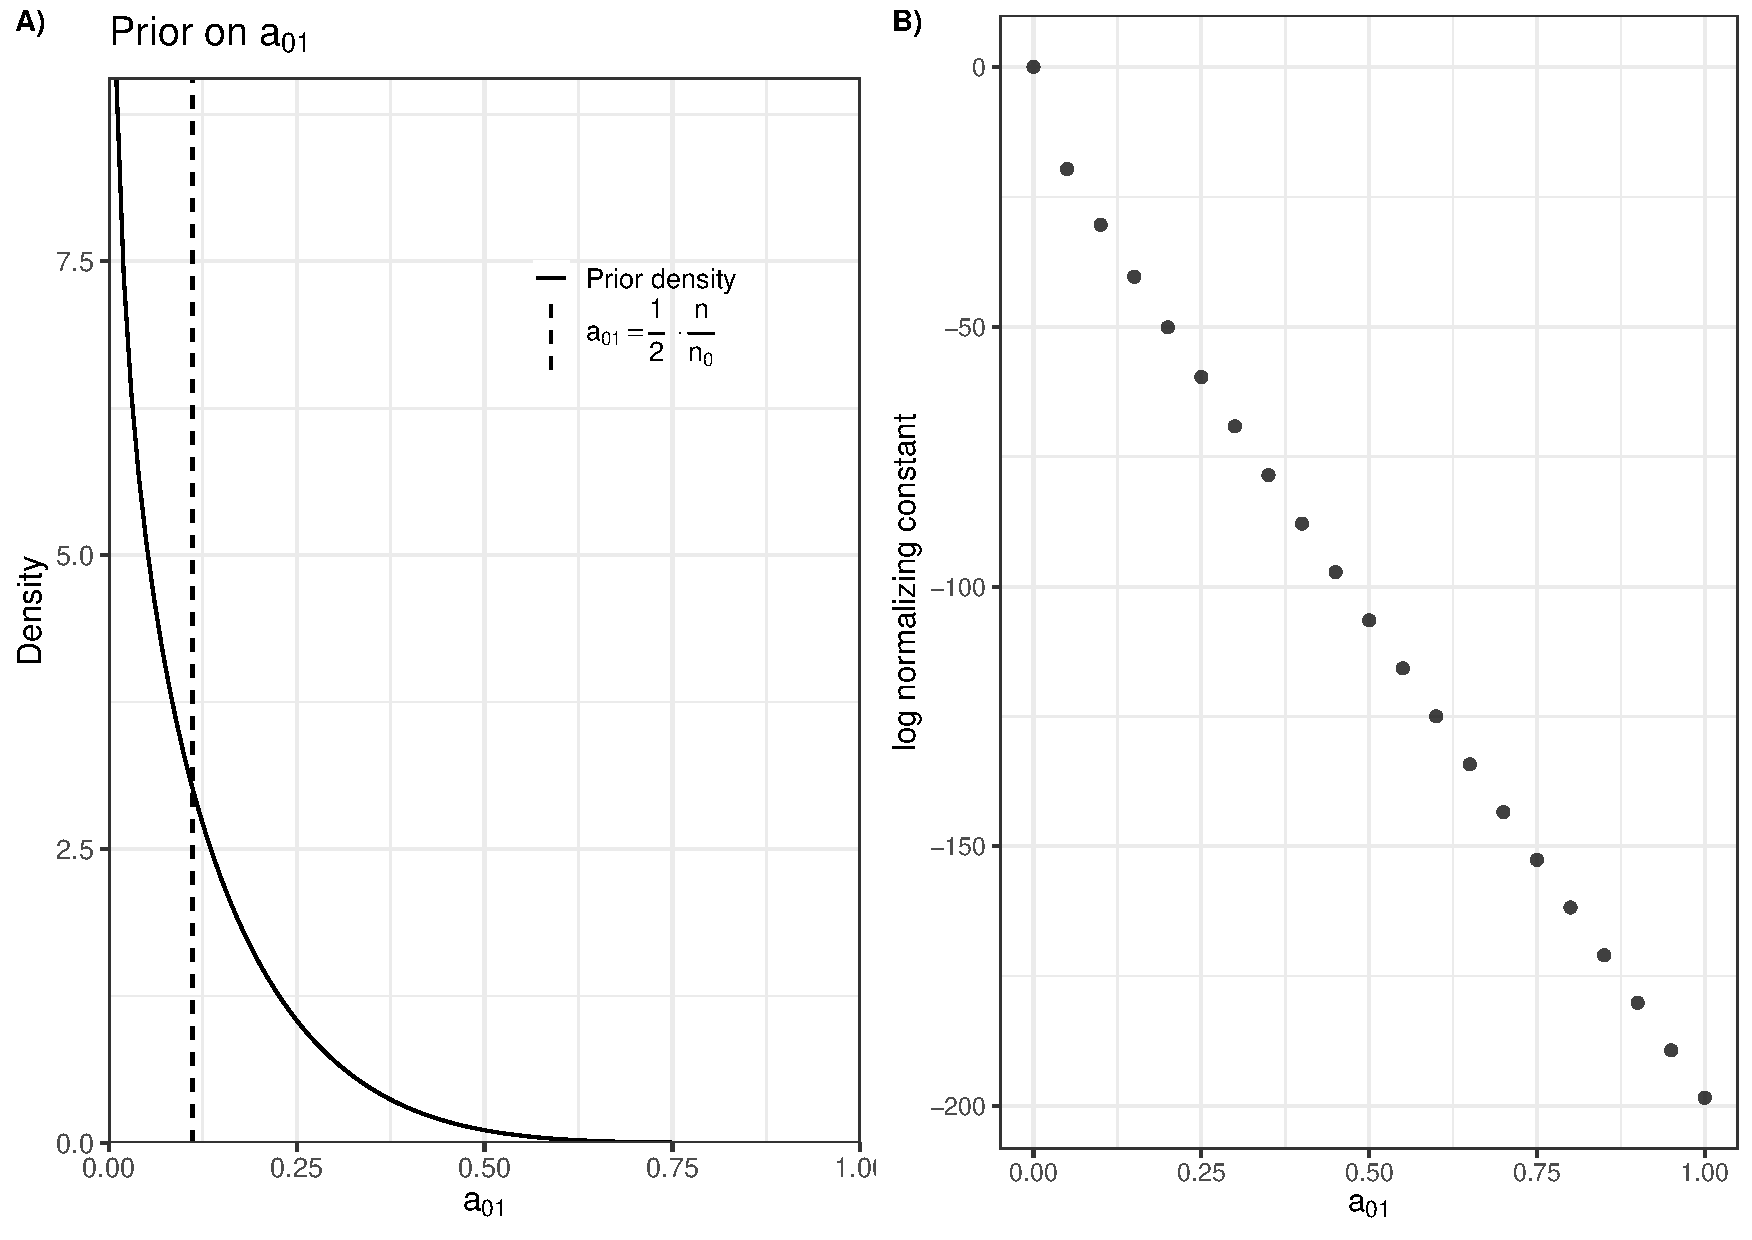
\includegraphics[scale=0.45]{figures/prior_and_normconst.pdf}
\caption{\label{fig:a0_prior_and_normconst}
\textbf{Beta prior distribution for $a_{01}$ and estimated log-normalizing constants as a function of $a_{01}$ for the AIDS progression logistic regression model.}
In panel A, the vertical dotted line marks the mean value $1/2 (n/n_0)$. Panel B shows the estimated log-normalizing constant obtained using Algorithm~\ref{alg:npp}.
Note that $\log Z_h(0) = 0$ for all $h$.
}
\end{figure}

As discussed in Section~\hyperref[sec:npp]{2.3}, implementing the NPP also requires estimating the normalizing constant $Z_1(a_{01})$ at several values of $a_{01}$ in order to approximately sample from the joint posterior of $a_{01}$ and $\boldsymbol{\theta}$, the model parameters.
Fortunately, this task can be accomplished in parallel using the \CRANpkg{parallel} package:
\begin{verbatim}
a0       <- seq(0, 1, length.out = 21)
histdata <- the.data[[2]]
## wrapper to obtain log normalizing constant in parallel package
logncfun <- function(a0, ...){
  hdbayes::glm.npp.lognc(
    formula = formula, family = family, histdata = histdata, a0 = a0, ...
  )
}
cl <- makeCluster(10)
clusterSetRNGStream(cl, 123)
clusterExport(cl, varlist = c('formula', 'family', 'histdata'))
## call created function
a0.lognc <- parLapply(
  cl = cl, X = a0, fun = logncfun, iter_warmup = 2*iter_warmup,
  iter_sampling = 2*iter_sampling, chains = nchains, refresh = 0
)
stopCluster(cl)
\end{verbatim}
Here, we specify a longer warm-up period to improve convergence for small values of $a_{01}$, which can lead to flatter posteriors that are more challenging to sample from.
The resulting \code{data.frame} includes the values of $a_{01}$, the corresponding estimated log-normalizing constants, and MCMC diagnostics, allowing users to assess the reliability of the results.

\begin{verbatim}
a0.lognc <- data.frame( do.call(rbind, a0.lognc) )
head(a0.lognc) %>%
    mutate(across(where(is.numeric), round, 3))

    a0   lognc min_ess_bulk max_Rhat
1 0.00   0.000    10492.866    1.001
2 0.05 -19.658     7016.144    1.001
3 0.10 -30.372     6495.816    1.001
4 0.15 -40.382     5753.908    1.001
5 0.20 -50.115     6753.503    1.001
6 0.25 -59.686     6865.135    1.001

\end{verbatim}
Figure~\ref{fig:a0_prior_and_normconst}B displays the estimated log-normalizing constants evaluated at a grid of 21 equally-spaced values of $a_{01} \in [0, 1]$. We are now ready to fit the NPP using the computations stored in \code{a0.lognc}.
\begin{verbatim}
fit.npp <- glm.npp(
  formula = formula, family = family, data.list = the.data,
  a0.lognc = a0.lognc$a0,
  lognc = matrix(a0.lognc$lognc, ncol = 1),
  a0.shape1 = beta.pars$a, a0.shape2 = beta.pars$b, ## Beta prior on a_{01}
  iter_warmup = iter_warmup, iter_sampling = iter_sampling,
  chains = nchains, parallel_chains = ncores,
  refresh = 0
)
get_summaries(fit = fit.npp, pars.interest = c(base.pars, "a0_hist_1"))

# A tibble: 6 × 6
  variable      mean    sd `2.5%`  `50%` `97.5%`
  <chr>        <dbl> <dbl>  <dbl>  <dbl>   <dbl>
1 (Intercept) -3.836 1.179 -6.546 -3.709  -1.932
2 age          0.278 0.265 -0.251  0.279   0.781
3 race         0.802 1.170 -1.166  0.690   3.437
4 treatment   -0.539 0.534 -1.594 -0.546   0.529
5 cd4         -1.193 0.339 -1.944 -1.158  -0.615
6 a0_hist_1    0.187 0.115  0.050  0.158   0.478  
\end{verbatim}
The NAPP (Section~\hyperref[sec:napp]{2.4}) can be fitted using very similar syntax:
\begin{verbatim}
fit.napp <- glm.napp(
  formula = formula, family = family, data.list = the.data,
  a0.shape1 = beta.pars$a, a0.shape2 = beta.pars$b,
  iter_warmup = iter_warmup, iter_sampling = iter_sampling,
  chains = nchains, parallel_chains = ncores,
  refresh = 0
)
get_summaries(fit = fit.napp, pars.interest = c(base.pars, "a0_hist_1"))

# A tibble: 6 × 6
  variable      mean    sd `2.5%`  `50%` `97.5%`
  <chr>        <dbl> <dbl>  <dbl>  <dbl>   <dbl>
1 (Intercept) -3.644 1.173 -6.204 -3.541  -1.645
2 age          0.302 0.252 -0.202  0.306   0.780
3 race         0.729 1.167 -1.288  0.632   3.234
4 treatment   -0.543 0.503 -1.530 -0.547   0.468
5 cd4         -1.113 0.322 -1.840 -1.081  -0.568
6 a0_hist_1    0.188 0.128  0.026  0.158   0.502
\end{verbatim}
Note that no reference to \code{a0.lognc} or \code{lognc} is necessary, as the normalizing constant for the NAPP is known in closed form. 

As described in Section~\hyperref[sec:LEAP]{2.8}, fitting the LEAP requires specifying the hyperparameters $K$ and $\bm{\alpha}_0$, corresponding to the arguments \code{K} and \code{prob.conc} in the \code{glm.leap()} function. Posterior samples under the LEAP can be obtained as follows:
\begin{verbatim}
fit.leap <- glm.leap(
  formula = formula, family = family, data.list = the.data,
  K = 2, prob.conc = rep(1, 2),
  iter_warmup = iter_warmup, iter_sampling = iter_sampling,
  chains = nchains, parallel_chains = ncores,
  refresh = 0
)
get_summaries(fit = fit.leap, pars.interest = c(base.pars, "gamma"))

# A tibble: 6 × 6
  variable      mean    sd `2.5%`  `50%` `97.5%`
  <chr>        <dbl> <dbl>  <dbl>  <dbl>   <dbl>
1 (Intercept) -4.206 1.025 -6.432 -4.083  -2.643 
2 age          0.300 0.183 -0.077  0.305   0.645 
3 race         1.154 1.021 -0.415  1.038   3.434
4 treatment   -0.668 0.425 -1.507 -0.680   0.228
5 cd4         -0.941 0.256 -1.507 -0.916  -0.514 
6 gamma        0.948 0.059  0.763  0.966  0.997

\end{verbatim}
In the output above, \code{gamma} represents the posterior probability that an individual in the historical data set is exchangeable with those in the current data, which corresponds to $\gamma_1$ in \eqref{eq:leap}. The posterior mean of \code{gamma} suggests a high degree of exchangeability between the current and historical data sets.

We are now ready to compare the performance of all methods investigated here. A graphical summary of the posterior estimates is presented in Figure~\ref{fig:models}.
As shown in Figure \ref{fig:models}, there is considerable variation in the coefficient estimates across different methods.
For instance, both the BHM and the RMAP prior pull the estimated treatment effect more strongly towards the historical MLE than the NAPP and PP do; however, the opposite pattern occurs for the estimated coefficient of \code{cd4}.
For all covariates, the coefficients estimated under the LEAP are the closest to the historical MLEs. We note, however, that we did not limit the amount of borrowing for the LEAP, which could, in principle, be controlled by imposing a truncated prior on $\gamma_1$ in \eqref{eq:leap}. While some methods, such as the PP, lead to more uncertain estimates of the treatment effect, the BHM and LEAP yield smaller uncertainties.
Importantly, all credible intervals include zero, indicating that despite incorporating information from a historical study with a significant treatment effect, the analysis of the current data suggests that the treatment effect could be null.

\begin{figure}[!ht]
\centering
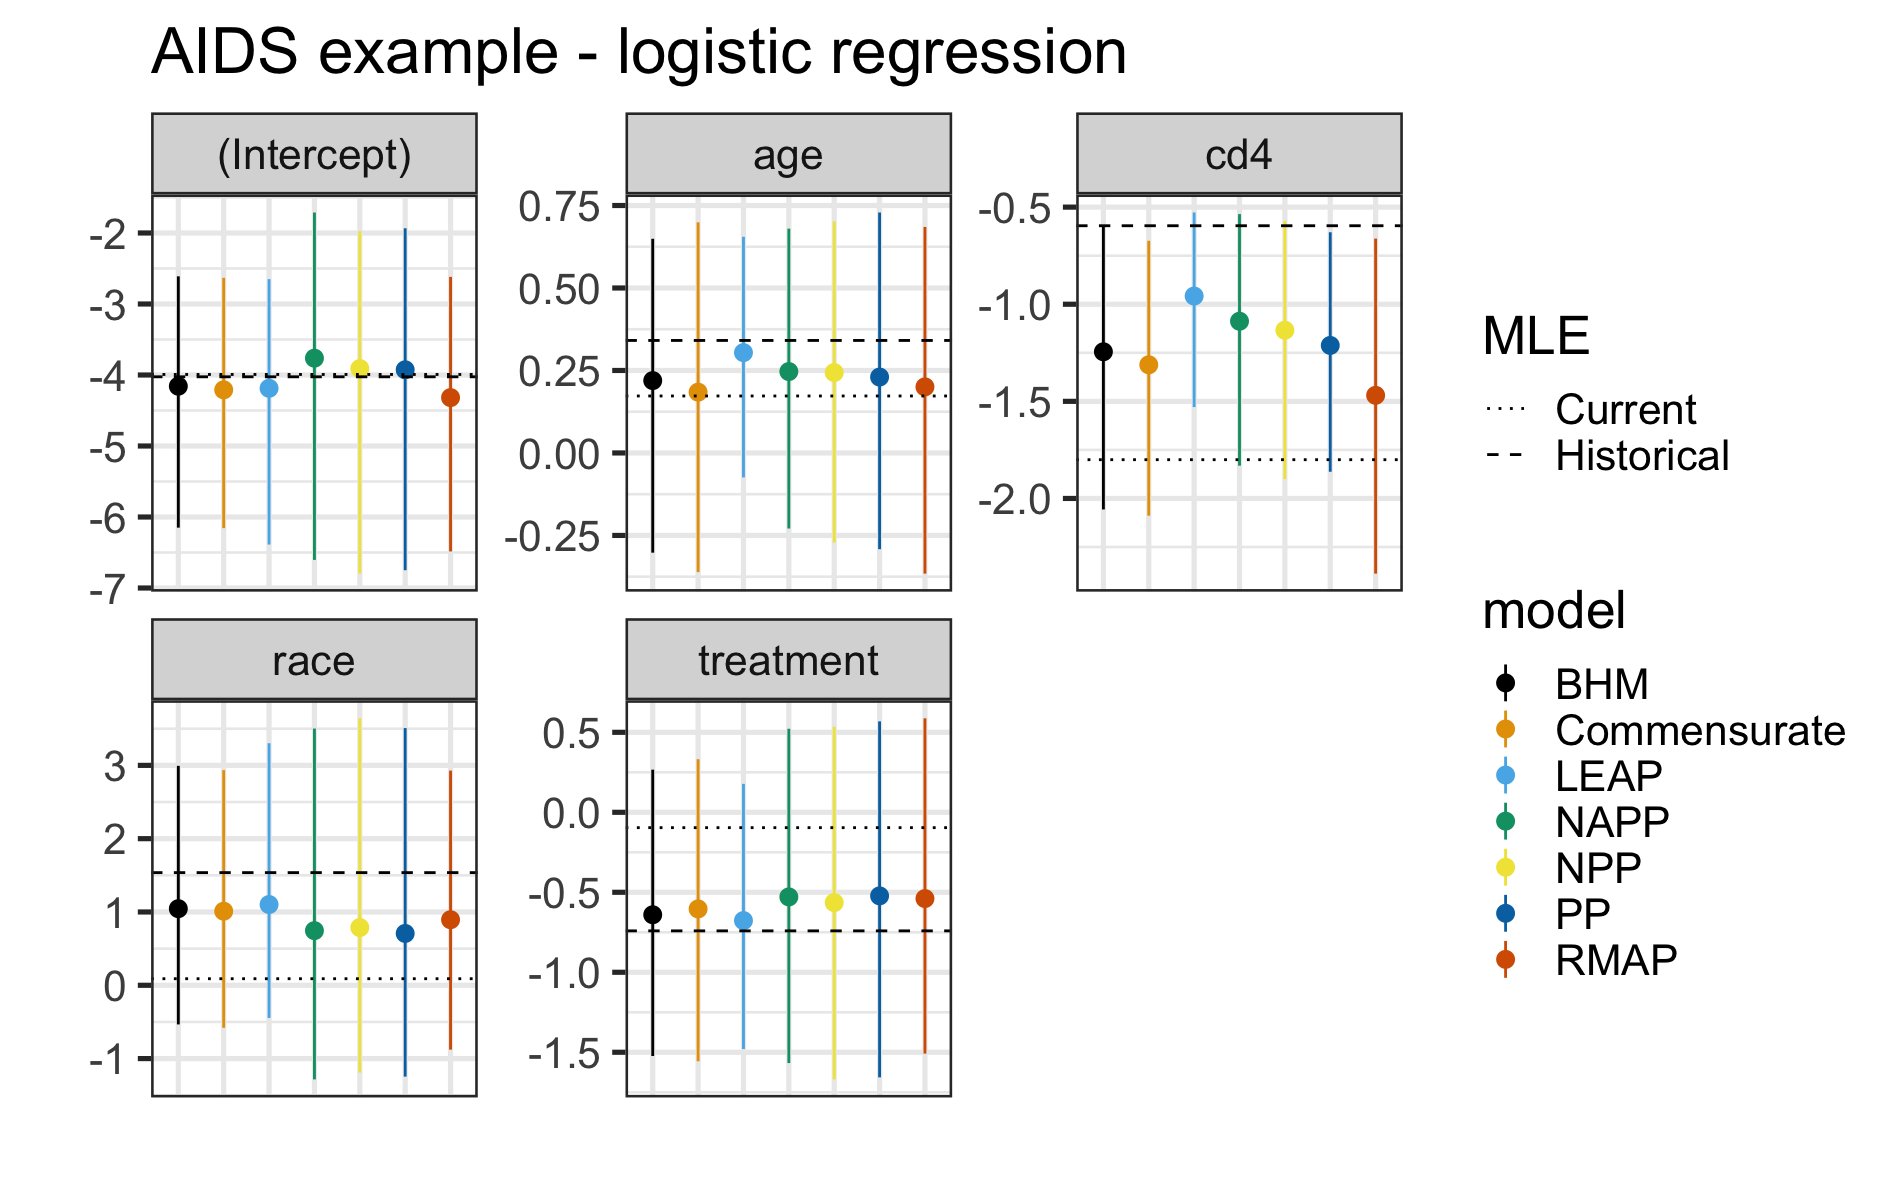
\includegraphics[width=\linewidth]{figures/posterior_estim.png}
\caption{\label{fig:models}
\textbf{Coefficient estimates for the AIDS progression logistic regression model}.
For each coefficient (vertical panels), we show the posterior mean (dot) and the $95\%$ equal-tailed credible interval (solid vertical line) for each of the models considered.
Horizontal lines (dotted: ACTG036; dashed: ACTG019) indicate the MLE for each coefficient.}
\end{figure}

\section{Discussion}
\label{sec:discussion}
The package \CRANpkg{hdbayes} provides a cohesive and user-friendly framework for implementing commonly used priors that incorporate historical data within GLMs. In addition, \CRANpkg{hdbayes} supports several survival models, including the PWEPH model, AFT models, and a mixture cure rate model, although we primarily focus on analyses using GLMs in this paper. The full suite of GLMs and link functions available in the \CRANpkg{stats} package is supported in \CRANpkg{hdbayes}, addressing an important gap in existing statistical software.

In the future, we aim to make several extensions to the \CRANpkg{hdbayes} package. For example, more complex data types (e.g., longitudinal data) could be included. Moreover, we aim to accommodate more flexible types of borrowing, such as partial borrowing techniques and methods for handling missing data. Finally, other types of historical data priors, such as propensity score-integrated priors, could be included to provide a comprehensive suite of tools for Bayesian dynamic borrowing within a single package.

\bibliography{hdbayes_RJ}

\address{Ethan M. Alt\\
  University of North Carolina at Chapel Hill\\
  135 Dauer Drive, Chapel Hill, NC\\
  USA\\
  ORCiD: 0000-0002-6112-9030\\
  \email{ethanalt@live.unc.edu}}

\address{Xinxin Chen\\
  University of North Carolina at Chapel Hill\\
  135 Dauer Drive, Chapel Hill, NC\\
  USA\\
  ORCiD: 0000-0003-1759-7811\\
  \email{xchen2.unc.edu}}

\address{Luiz M. Carvalho\\
  Getulio Vargas Foundation\\
  Rio de Janeiro \\
  Brazil\\
  \email{lmax.fgv@gmail.com}}

\address{Joseph G. Ibrahim\\
  University of North Carolina at Chapel Hill\\
  135 Dauer Drive, Chapel Hill, NC\\
  USA\\
  \email{ibrahim@bios.unc.edu}}

\newpage

\appendix

\setcounter{figure}{0}
\setcounter{table}{0}
\renewcommand{\thetable}{S\arabic{table}}
\renewcommand{\thefigure}{S\arabic{figure}}

\section*{ A. Link selection in binary regression with the power prior}
\label{sec:app_link_selection}

When employing GLMs, the choice of link function can be crucial, as it controls the degree of non-linearity between the conditional mean and the linear predictor. Here we illustrate how to use \CRANpkg{hdbayes} to compute marginal likelihoods (and thus Bayes factors) under the PP, comparing the logit and probit links in a binary regression model.

Let $\boldsymbol{y}_0$ and $\boldsymbol{y}$ denote the historical and current binary response vectors, respectively. We compare the following logistic and probit models for the probability $\mu_i$ that $y_i = 1$:
\begin{align}
\mathcal{M}_1&: \mu_i = \frac{\exp\left(\bm{x}_i'\bm{\beta}\right)}{1 + \exp\left(\bm{x}_i'\bm{\beta}\right)},\\
\mathcal{M}_2&:  \mu_i = \Phi\left(\bm{x}_i'\bm{\beta}\right),
\end{align}
where $\Phi$ is the cumulative distribution function of a standard normal random variable. We use the PP with a fixed discounting parameter $a_0$ to elicit priors for both models and employ bridge sampling to approximate the marginal likelihoods for $i = 1, 2$:
\begin{align}
    \label{eq:posterior_mal}
    m_i(a_0) &:=  \int_{\mathbb{R}^p} L_i(\bm{\beta} | D) \pi_{\text{PP}}(\bm{\beta} | D_{0}, a_{0}, \pi_0, \mathcal{M}_i) ~d\bm{\beta},\\
    \label{eq:prior_mal}
    \pi_{\text{PP}}(\bm{\beta} | D_{0}, a_{0}, \pi_0, \mathcal{M}_i) &:= \frac{L_i(\bm{\beta} | D_0)^{a_0}\pi_0(\bm{\beta})}{ \int_{\mathbb{R}^p} L_i(\bm{\beta} | D_0)^{a_0}\pi_0(\bm{\beta}) ~d\bm{\beta}},
\end{align}
where $D_0 = (\bm{y}_0, \bm{x}_0)$ and $D = (\bm{y}, \bm{x})$ denote the historical and current data sets, respectively, and $L_i$ and $\pi_{\text{PP}}(\cdot | \ldots, \mathcal{M}_i)$ are the likelihood and PP under model $\mathcal{M}_i$. For simplicity, we specify the same initial prior for the regression coefficients $\bm{\beta}$ in both models, assigning independent $N(0, 10^2)$ distributions, which correspond to the default prior in the PP implementation of \CRANpkg{hdbayes}.

Notice that this computation necessitates two passes of the bridge sampling algorithm: one to estimate the PP normalizing constant in \eqref{eq:prior_mal}, and another to estimate the normalizing constant of the posterior. The Bayes factor is then given by $\text{BF}_{12}(a_0) = m_1(a_0)/m_2(a_0)$.
It is interesting to understand how this quantity changes with different values of $a_0$ using the HIV data in Section~\hyperref[sec:dataanalysis_logistic]{4.1}.

We show the results in Figure~\ref{fig:link_selection}, where the logarithm of $\text{BF}_{12}(a_0)$ is plotted over a regular grid of discounting parameter values ranging from $a_0 = 0$ to $a_0 = 1$ in increments of $0.1$ is shown.
Following~\cite{kass1995bayes}, we mark the $\text{BF}_{12}(a_0) \geq 1$ (dashed) and $\text{BF}_{12}(a_0) \geq 3$ (dotted) which correspond to weak and substantial evidence, respectively (see Section 3.2 therein).
It is clear that the logit link is generally preferred over the probit link.
However, the relative support is not very strong, as evidenced by the fact that $\text{BF}_{12}(a_0) \geq 3$ is observed only for $a_0 < 0.1$.
This suggests that one would need to introduce very little borrowing in order to observe strong support for the logit link.

\begin{figure}[ht]
\centering
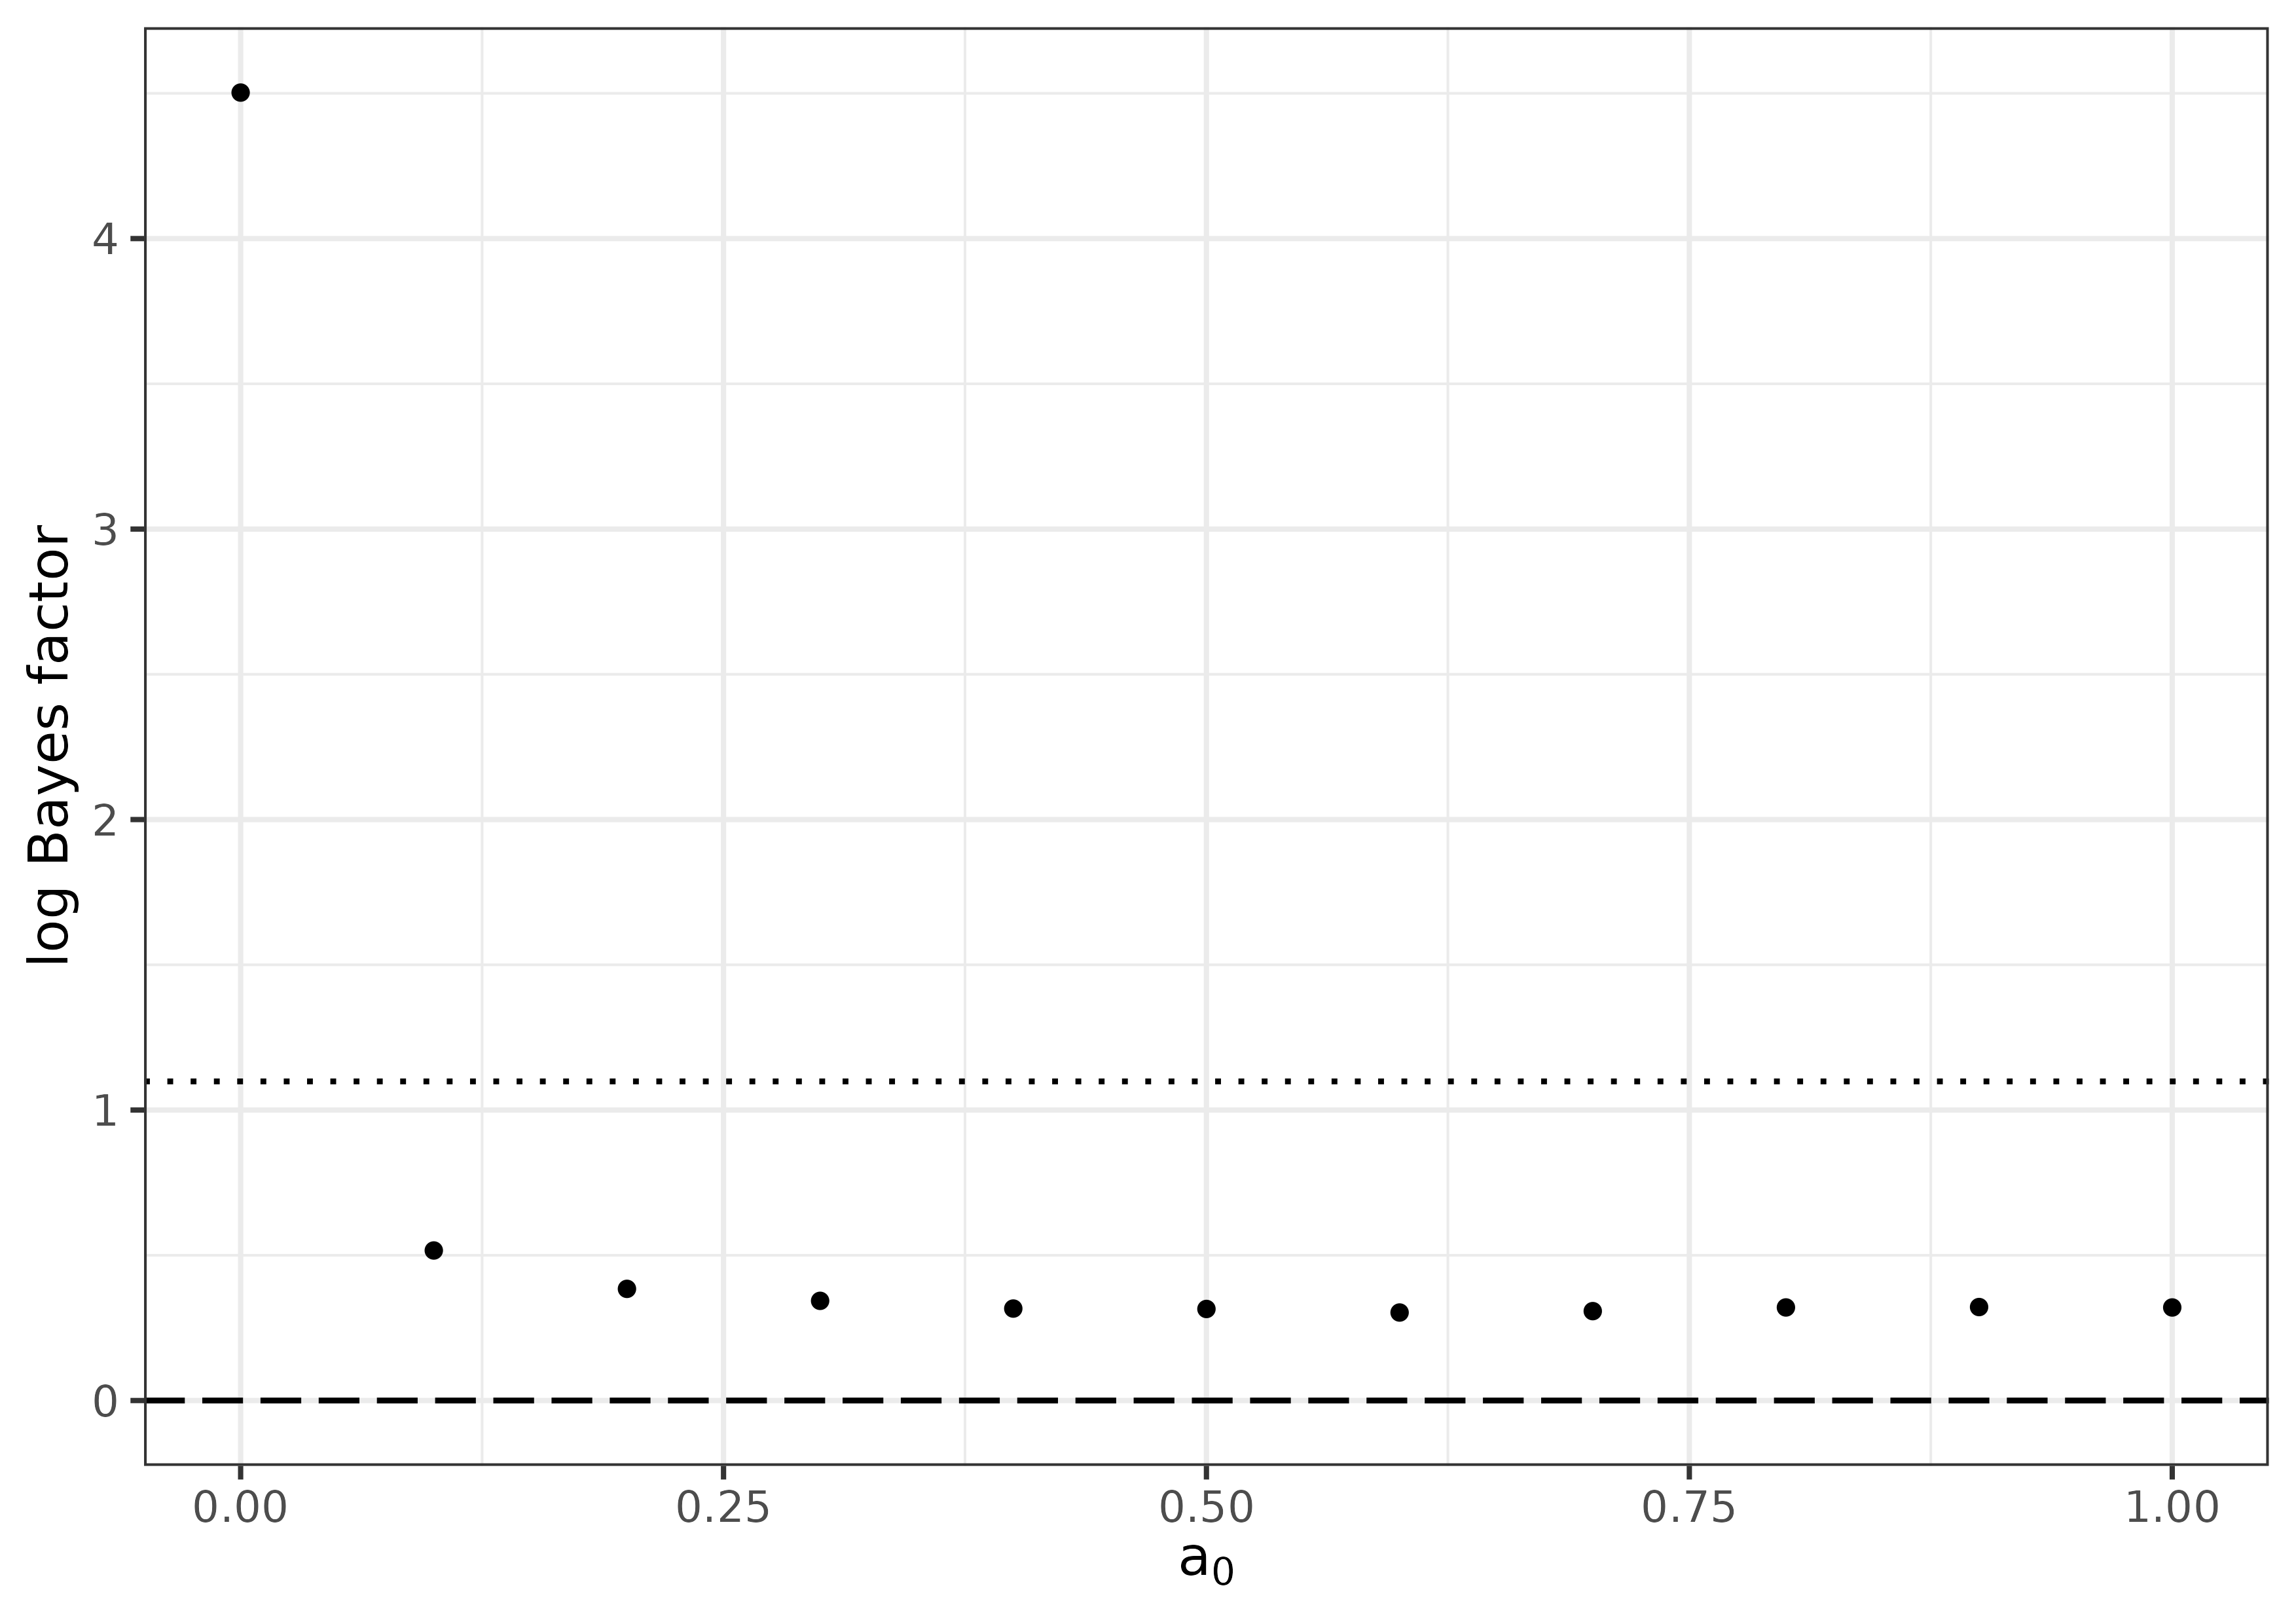
\includegraphics[scale=0.35]{figures/a0_logZ.png}
\caption{\label{fig:link_selection}
\textbf{Log Bayes factor comparing logit (Model 1, $\mathcal{M}_1$) and probit ($\mathcal{M}_2$) links for various values of the discounting parameter $a_0$}.
We show $\log\left(m_1(a_0)/m_2(a_0)\right)$.
Horizontal lines mark the $\log\text{BF}_{12} \geq 0$ (dashed) and $\log \text{BF}_{12} \geq \log(3) $ (dotted) thresholds.
}
\end{figure}

% To further explore this behavior, we repeat the above analysis for a regular grid of values from $a_0 = 0$ to $a_0 = 10^{-3}$.
% We see that the Bayes factor crosses the $\text{BF} \geq 3$ line at $a_0 \approx 5 \times 10^{-4}$. 
% This confirms that to obtain strong support for the logit model, one would need to discount the historical data much more strongly than one would usually consider.

% \begin{figure}[ht]
% \centering
% \includegraphics[scale=0.35]{figures/a0_logZ_zoom.png}
% \caption{\label{fig:link_selection_zoom}
% \textbf{Log Bayes factor comparing logit (Model 1, $\mathcal{M}_1$) and probit ($\mathcal{M}_2$) for small values of the discounting parameter $a_0$}.
% See Figure~\ref{fig:link_selection_zoom}.
% }
% \end{figure}
